\begin{English}
\section{Software}
\end{English}

\begin{Czech}
\section{Software}
\end{Czech}


\begin{English}
The system is accessible from IP adress \url{http://192.168.11.196:8123}.  Any current web browser is sufficient. It is possible to use mobile application for Android, download from Play Store.
\end{English}

\begin{Czech}
Systém je přístupný na IP adrese \url{http://192.168.11.196:8123}. Stačí jakýkoliv aktuální webový prohlížeč. Je možné využít i mobilní aplikaci na Android, stažení přímo v Play Store.
\end{Czech}


% ====================  START Overview Tab  ====================
\begin{English}
\subsection{The Overview tab}
\end{English}

\begin{Czech}
\subsection{Záložka přehled}
\end{Czech}


\begin{English}
In a \textbf{Overview} tab (the picture \ref{fig:overview-tab} – a blue top menu) can be seen in one chart in a part "Comparison of Temperatures" all measured temperatures (fireplaces, tank of heat water and outside temperature). In a part "\textit{Individual Sensors}", are individual temeperature sensors with current measured temperature.
\end{English}

\begin{Czech}
V záložce \textbf{přehled} (obrázek \ref{fig:overview-tab} – horní modré menu) jsou vidět v jednom grafu v části „Porovnání teploty“ všechny měřené teploty (krby, zásobník otopné vody a venkovní teplota). V části „\textit{Jednotlivé senzory}“ jsou jednotlivé teplotní senzory s aktuálně naměřenou teplotou. 
\end{Czech}


\begin{English}
\begin{figure}[H]
    \centering
    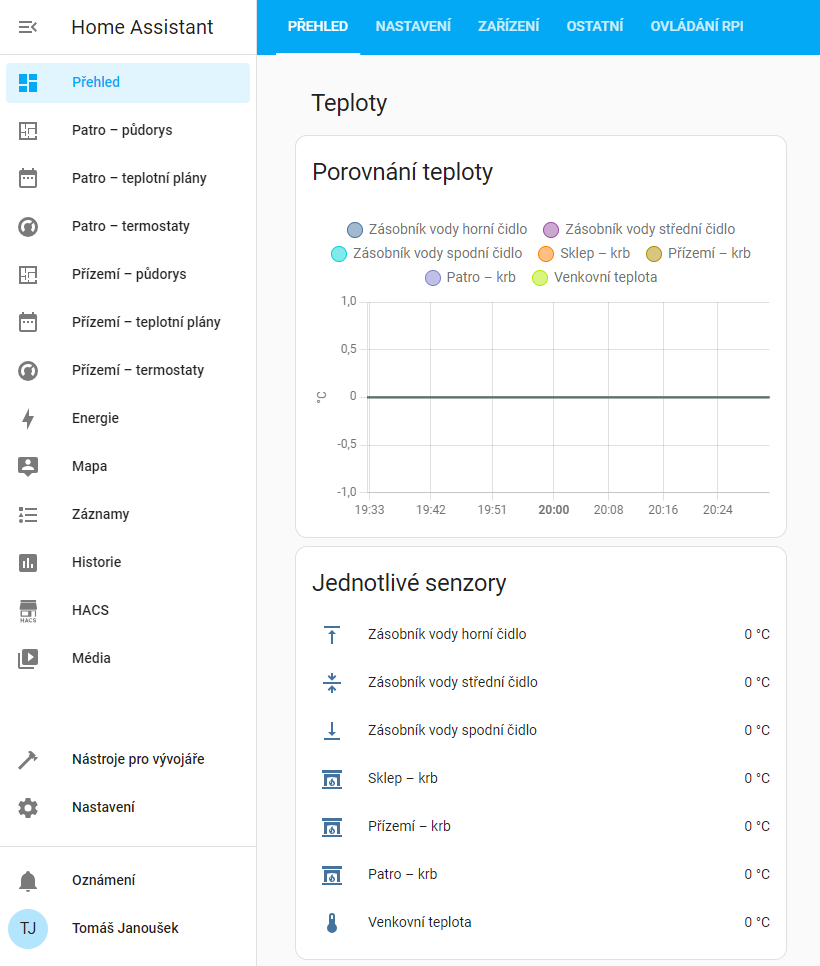
\includegraphics[width=0.9\textwidth]{pictures/czech/software/overview-tab.png}
    \caption{The Overview tab.}
    \label{fig:overview-tab}
\end{figure}
\end{English}

\begin{Czech}
\begin{figure}[H]
    \centering
    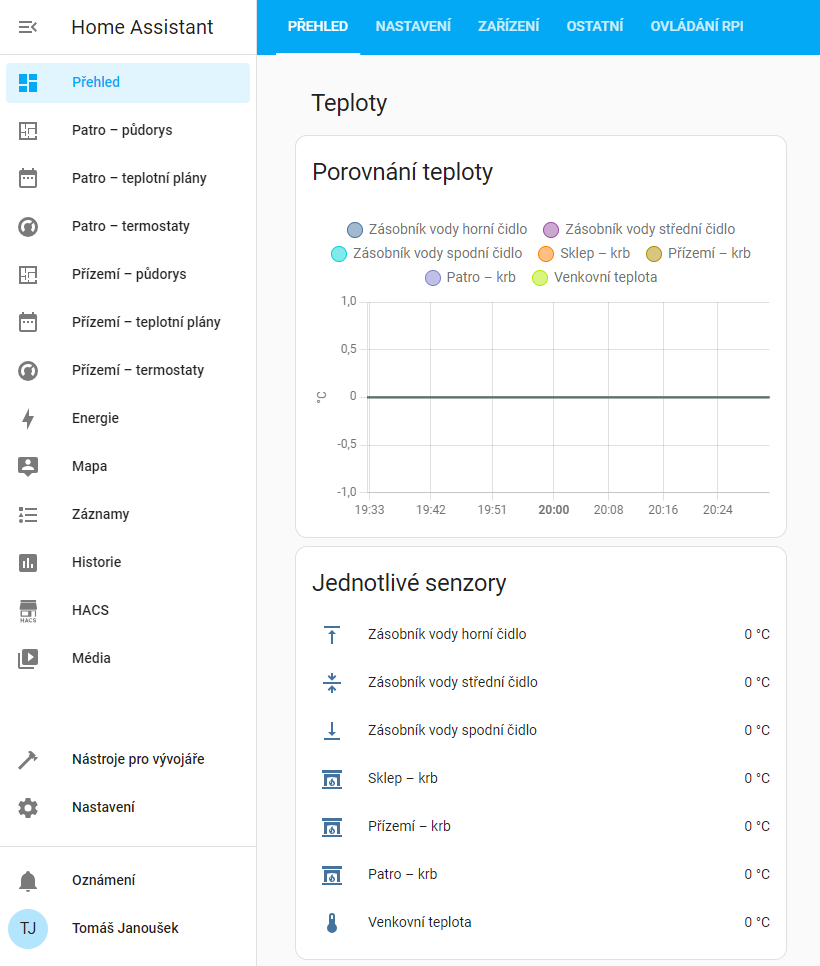
\includegraphics[width=0.9\textwidth]{pictures/czech/software/overview-tab.png}
    \caption{Záložka přehled.}
    \label{fig:overview-tab}
\end{figure}
\end{Czech}


\begin{English}
If user clicks on a name of temperature sensor (for example, the Tank with Water Top Sensor) then the history of measured values is displayed (the figure \ref{fig:click-temperature-sensor}). 
Double-clicking on the top part of this window will further enlarge the displayed window. 
\end{English}

\begin{Czech}
Pokud uživatel klikne na název teplotního senzoru (např. Zásobník vody horní čidlo), zobrazí se historie naměřených hodnot (obrázek \ref{fig:click-temperature-sensor}). Dvojitým kliknutí na horní část tohoto okna se zobrazené okno ještě zvětší.
\end{Czech}


\begin{English}
\begin{figure}[H]
    \centering
    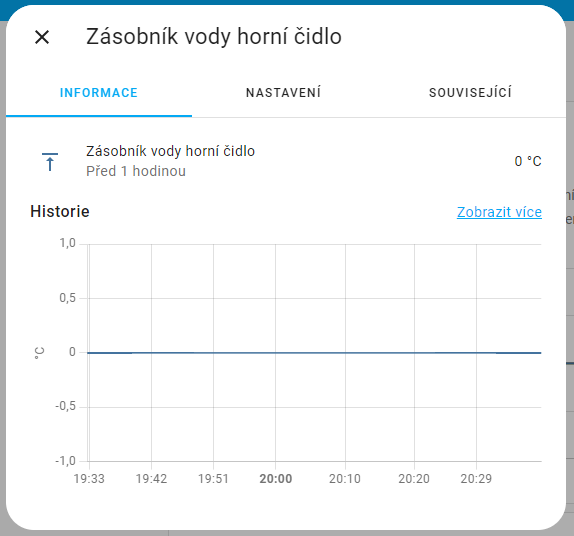
\includegraphics[width=0.6\textwidth]{pictures/czech/software/click-temperature-sensor.png}
    \caption{The temperature sensor history is displayed after clicking on its name.}
    \label{fig:click-temperature-sensor}
\end{figure}
\end{English}

\begin{Czech}
\begin{figure}[H]
    \centering
    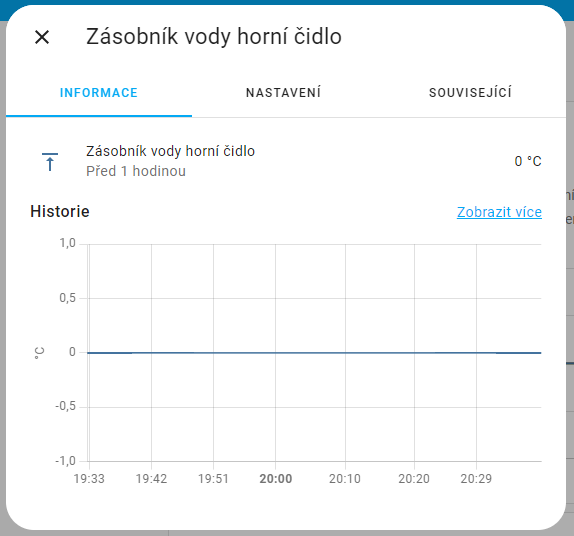
\includegraphics[width=0.6\textwidth]{pictures/czech/software/click-temperature-sensor.png}
    \caption{Zobrazení historie senzoru teplotu po kliknutí na název.}
    \label{fig:click-temperature-sensor}
\end{figure}
\end{Czech}
% ====================  STOP Overview Tab  ====================

% ====================  START Settings Tab  ====================
\begin{English}
\subsection{The settings tab}
\end{English}

\begin{Czech}
\subsection{Záložka nastavení}
\end{Czech}

\begin{English}
In a \textbf{Settings} tab (the figure \ref{fig:settings-tab} – top blue menu) are displayed modes "\textit{Control of Temperature}", "\textit{Control Modes}", "\textit{Switching Heat Coil}", "\textit{Fireplaces – Switching of Pumps}", "\textit{LED Indication – Limit Parameters of Hot Water Tank}" and "\textit{Other Settings}". Individual options are described below.
\end{English}

\begin{Czech}
V záložce \textbf{nastavení} (obrázek \ref{fig:settings-tab} – horní modré menu) jsou vidět módy „\textit{Řízení teploty}“, „\textit{Módy řízení}“, „\textit{Spínání topné spirály}“, „\textit{Krby – spínání čerpadel}“, „\textit{LED indikace – mezní parametry zásobníku teplé vody}“ a „\textit{Ostatní nastavení}“. Jednotlivé možnosti jsou popsány níže.
\end{Czech}


\begin{English}
\begin{figure}[H]
    \centering
    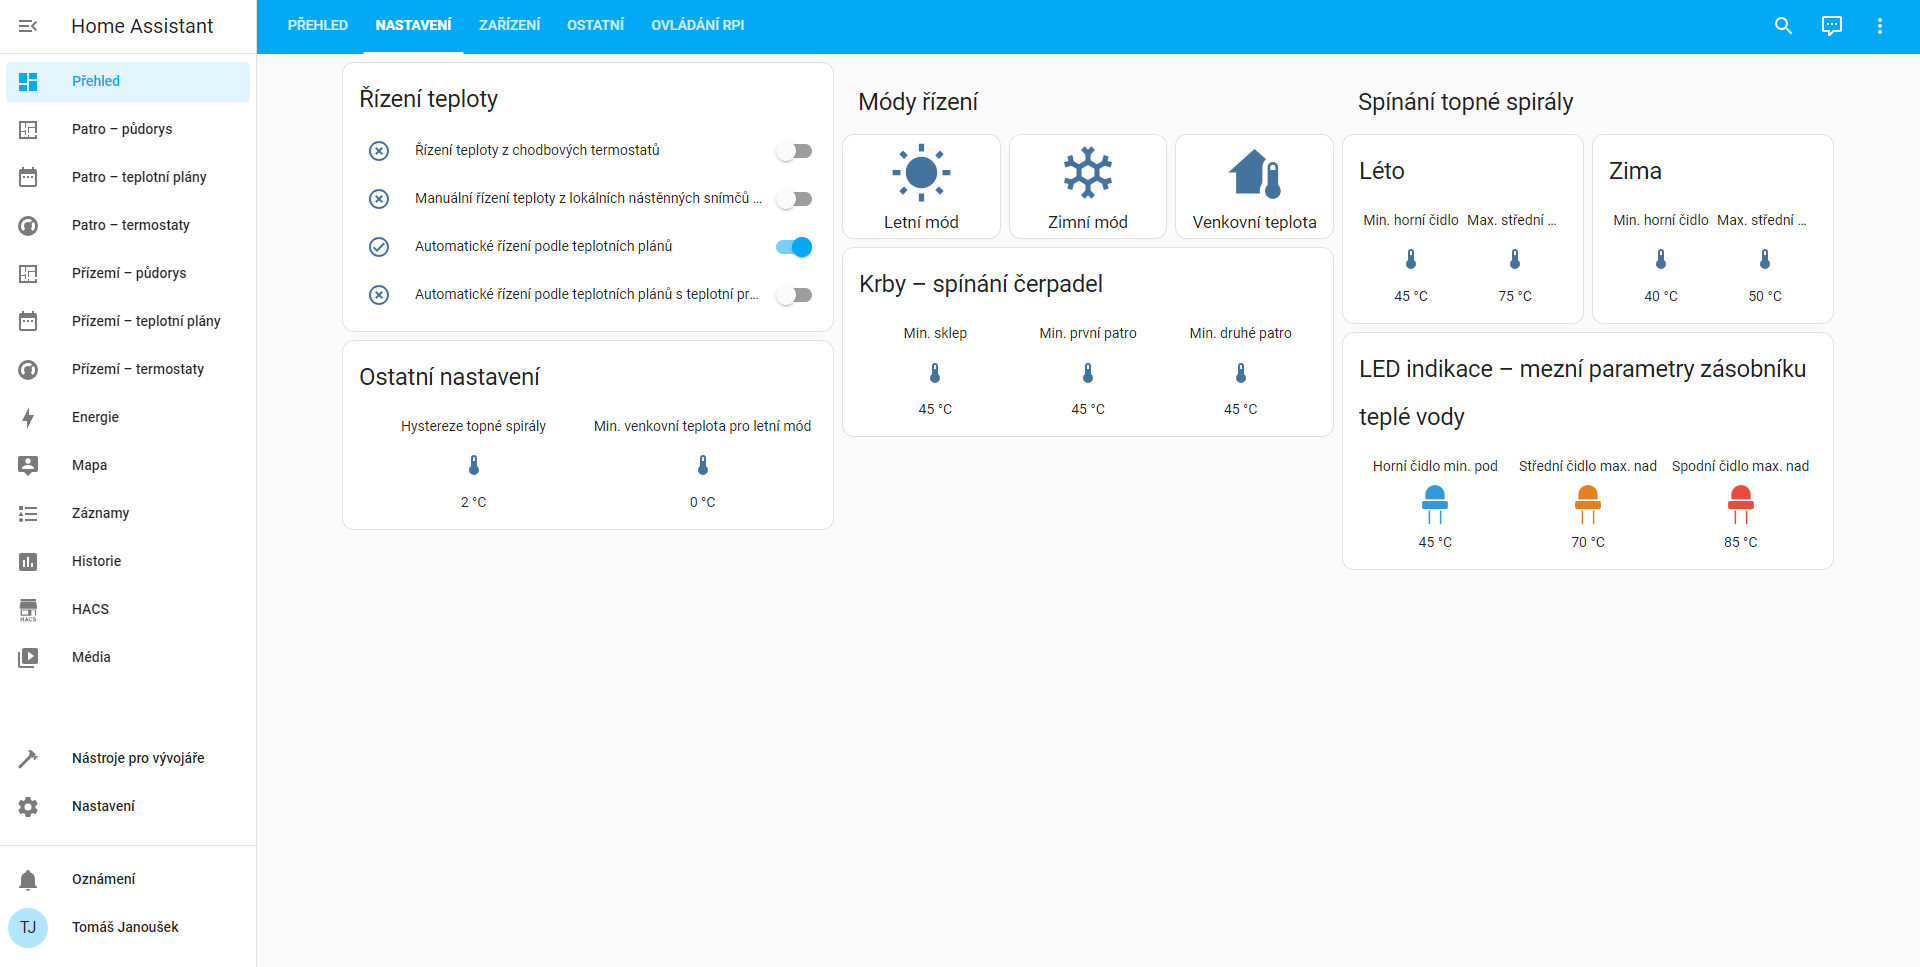
\includegraphics[width=1\textwidth]{pictures/czech/software/settings-tab.png}
    \caption{The Settings tab.}
    \label{fig:settings-tab}
\end{figure}
\end{English}

\begin{Czech}
\begin{figure}[H]
    \centering
    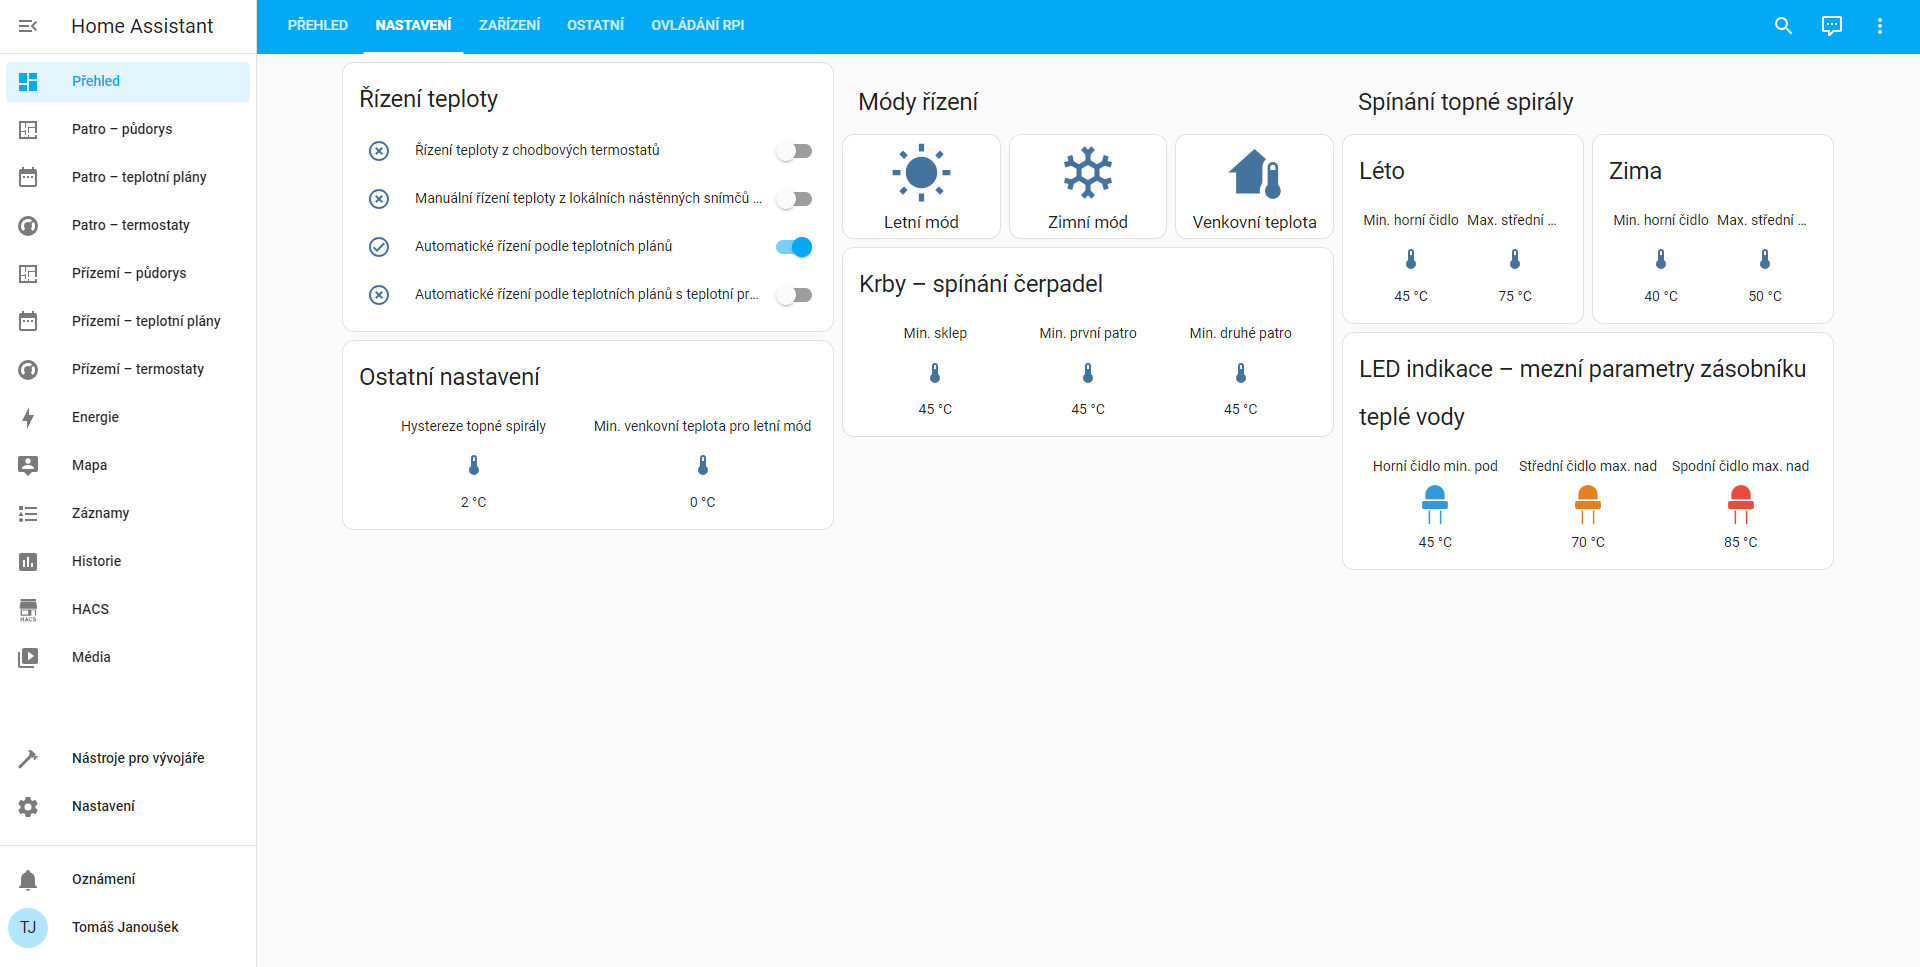
\includegraphics[width=1\textwidth]{pictures/czech/software/settings-tab.png}
    \caption{Záložka nastavení.}
    \label{fig:settings-tab}
\end{figure}
\end{Czech}

% ========================================

\begin{English}
\subsubsection{Temperature control}
\end{English}

\begin{Czech}
\subsubsection{Teplotní řízení}
\end{Czech}
\label{sec:temperature-control}


\begin{English}
In the section of settings "\textit{Temperature Control}" (the figure \ref{fig:temperature-control}) is possible to select from several modes. In order to control heating, it is necessary to always select one of the control modes, otherwise, the heating will not be managed automatically according to automation.
\end{English}

\begin{Czech}
V části nastavení „\textit{Řízení teploty}“ (obrázek \ref{fig:temperature-control}) je možné vybrat z  několika módů. Pro řízení vytápění je nutné vždy vybrat jeden z módů řízení v opačném případě nebude docházet k řízení vytápění podle automatizace.
\end{Czech}


\begin{English}
\begin{figure}[H]
    \centering
    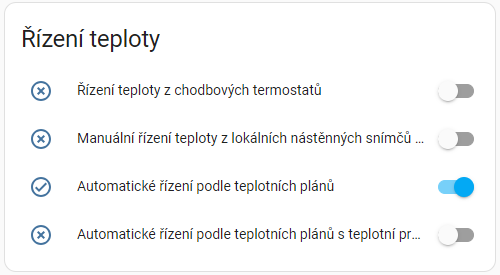
\includegraphics[width=0.6\textwidth]{pictures/czech/software/temperature-control.png}
    \caption{Temperature Control.}
    \label{fig:temperature-control}
\end{figure}
\end{English}

\begin{Czech}
\begin{figure}[H]
    \centering
    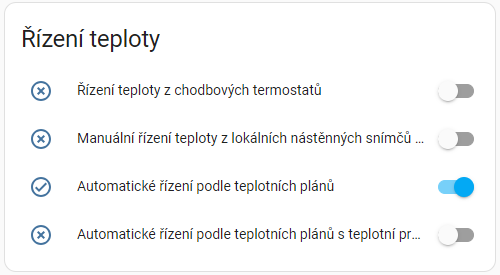
\includegraphics[width=0.6\textwidth]{pictures/czech/software/temperature-control.png}
    \caption{Řízení teploty.}
    \label{fig:temperature-control}
\end{figure}
\end{Czech}

% ========================================

\begin{English}
\subsubsubsection{Temperature Control from Corridor Thermostats}
\end{English}
\begin{Czech}
\subsubsubsection{Řízení teploty z chodbových termostatů}
\end{Czech}


\begin{English}
In a mode "\textit{Temperature Control from Corridor Thermostats}", the temperature settings in the corridor thermostats, located on the ground floor and on the first floor, determine the heating operation for all heating circuits on the respective floor. If there is request for heating, all heating circuits will be turned on otherwise will be turn off. The status of individual corridor thermostats (heating status) is indicated by a glowing red LED directly on the thermostat or within the system under the \textbf{Devices} tab in the section \textit{Corridor Thermostats – Heating Request} for each floor, as shown in the figure \ref{fig:corridor-thermostats}. The status of individual heating circuits is showed on the \textbf{Devices} tab in the section „\textit{The Ground Floor or the First Floor – Heating Circuits (Valves)}“, as shown in the figure \ref{fig:heating-circuits-ground-floor}.
\end{English}

\begin{Czech}
V módu „\textit{Řízení teploty z chodbových termostatů}“ docházení na základě nastavené teploty v chodbových termostatech, které jsou umístěné v přízemí a v patře k ovládání všech otopných okruhů pro dané patro. Pokud je požadavek na vytápění, dojde k zapnutí všechny otopných okruhů, jinak dojde k vypnutí. Stav zapnutí jednotlivých chodbových termostatů (stav vytápění) je signalizovány svítící červenou LED přímo na termostatu, případně v systému v \textbf{záložce zařízení} \mbox{v části} „\textit{Termostaty chodby – požadavek topení}“ pro každé patro, obrázek \ref{fig:corridor-thermostats}. Stav jednotlivých otopných okruhů je vidět na \textbf{záložce zařízení} v části „\textit{Přízení nebo patro – otopné okruhy (ventily)}“, obrázek \ref{fig:heating-circuits-ground-floor}.
\end{Czech}


\begin{English}
\begin{figure}[H]
    \centering
    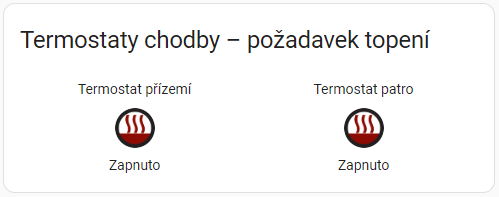
\includegraphics[width=0.6\textwidth]{pictures/czech/software/corridor-thermostats.png}
    \caption{Corridor Thermostats – Heating Request.}
    \label{fig:corridor-thermostats}
\end{figure}
\end{English}

\begin{Czech}
\begin{figure}[H]
    \centering
    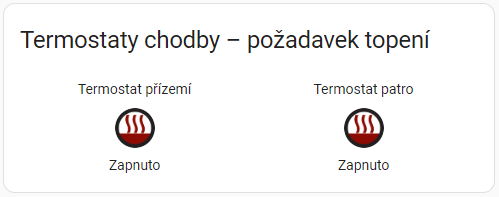
\includegraphics[width=0.6\textwidth]{pictures/czech/software/corridor-thermostats.png}
    \caption{Termostaty chodby – požadavek topení.}
    \label{fig:corridor-thermostats}
\end{figure}
\end{Czech}


\begin{English}
\begin{figure}[H]
    \centering
    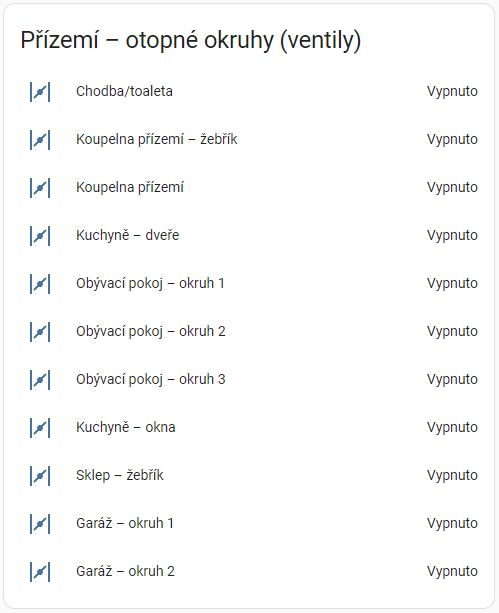
\includegraphics[width=0.6\textwidth]{pictures/czech/software/heating-circuits-ground-floor.png}
    \caption{The Ground Floor – Heating Circuits (Valves).}
    \label{fig:heating-circuits-ground-floor}
\end{figure}
\end{English}

\begin{Czech}
\begin{figure}[H]
    \centering
    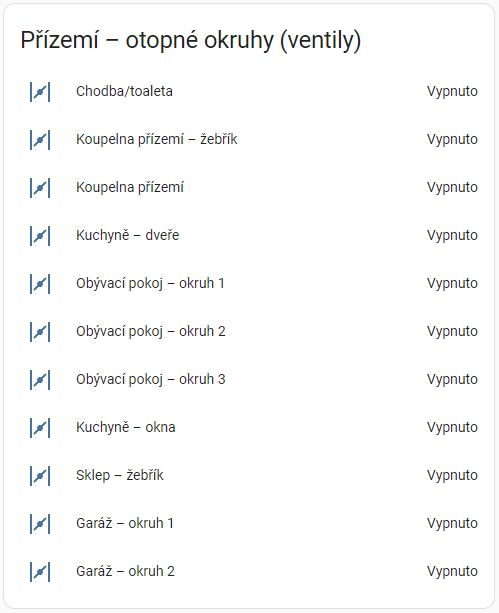
\includegraphics[width=0.6\textwidth]{pictures/czech/software/heating-circuits-ground-floor.png}
    \caption{Přízemí – otopné okruhy (ventily).}
    \label{fig:heating-circuits-ground-floor}
\end{figure}
\end{Czech}


\begin{English}
\tipbox{Attention!}{This control is working only if it is enable "Winter Mode" in the section "Mode Control". Further description in the section \ref{sec:control-modes} "Control Modes".}
\end{English}

\begin{Czech}
\tipbox{Pozor!}{Toto řízení je funkční jen v případě povolení „Zimní mód“ v části „Módy řízení“. Další popis v části \ref{sec:control-modes} „Módy řízení“.}
\end{Czech}

% ========================================

\begin{English}
\subsubsubsection{Manual Control of Temperature from Local Temperature Sensors}
\end{English}

\begin{Czech}
\subsubsubsection{Manuální řízení teploty z lokálních snímáčů teploty}
\end{Czech}


\begin{English}
In the mode "\textit{Manual Control of Temperature from Local Temperature Sensors}" is temperature control according to the given wall temperature sensor which is located in each room. For each room is control of heating circuits. The status individual thermostats are showed in the left menu under "\textit{The Ground Floor – thermostats}" or "\textit{The First Floor – thermostats}", as shown in the figure \ref{fig:thermostats-first-floor}. Each thermostat allows to set required temperature  using the orange slider (the figure \ref{fig:thermostat}), alternatively, it is possible to click on 3 dots in the top right corner of the thermostat and adjust the required temperature using the arrows, as shown the figure \ref{fig:click-thermostat}. The currently measured temperature is displayed in the middle. Beneath each thermostat, there is information "\textit{Connection Status}" which indicates connection of thermostat to system and "\textit{Detection of Open Window}" which indicates open window in a room. If window is open, heating is turned off for room with open window. If window is close, heating is restored.
\end{English}

\begin{Czech}
V módu „\textit{Manuální řízení teploty z lokálních snímáčů teploty}“ dochází k řízení teploty podle daného nástěnného snímače teploty umístěný v každé místnosti. Pro danou místnost jsou následně ovládány otopné okruhy. Stav jednotlivých termostatů je vidět v levém menu v „\textit{Přízemí – termostaty}“ nebo v „\textit{Patro – termostaty}“, obrázek \ref{fig:thermostats-first-floor}. Na každém termostatu (obrázek \ref{fig:thermostat}) lze nastavit požadovanou teplotu pomocí oranžového posuvníku, případně lze kliknout na 3 tečky v pravém horním rohu termostatu a požadovanou teplotu lze nastavit pomocí šipek, obrázek \ref{fig:click-thermostat}. Aktuálně naměřená teplota se zobrazuje uprostřed. Pod každým termostatem je dále informace „\textit{Stav připojení}“, která signalizuje, zda daný snímač je připojen do systému a „\textit{Detekce otevřeného okna}“, která signalizuje, zda došlo k otevření okna v místnosti, v takovém případě dojde k pozastavení vytápění pro danou místnost než se okno opět zavře.
\end{Czech}


\begin{English}
\begin{figure}[H]
    \centering
    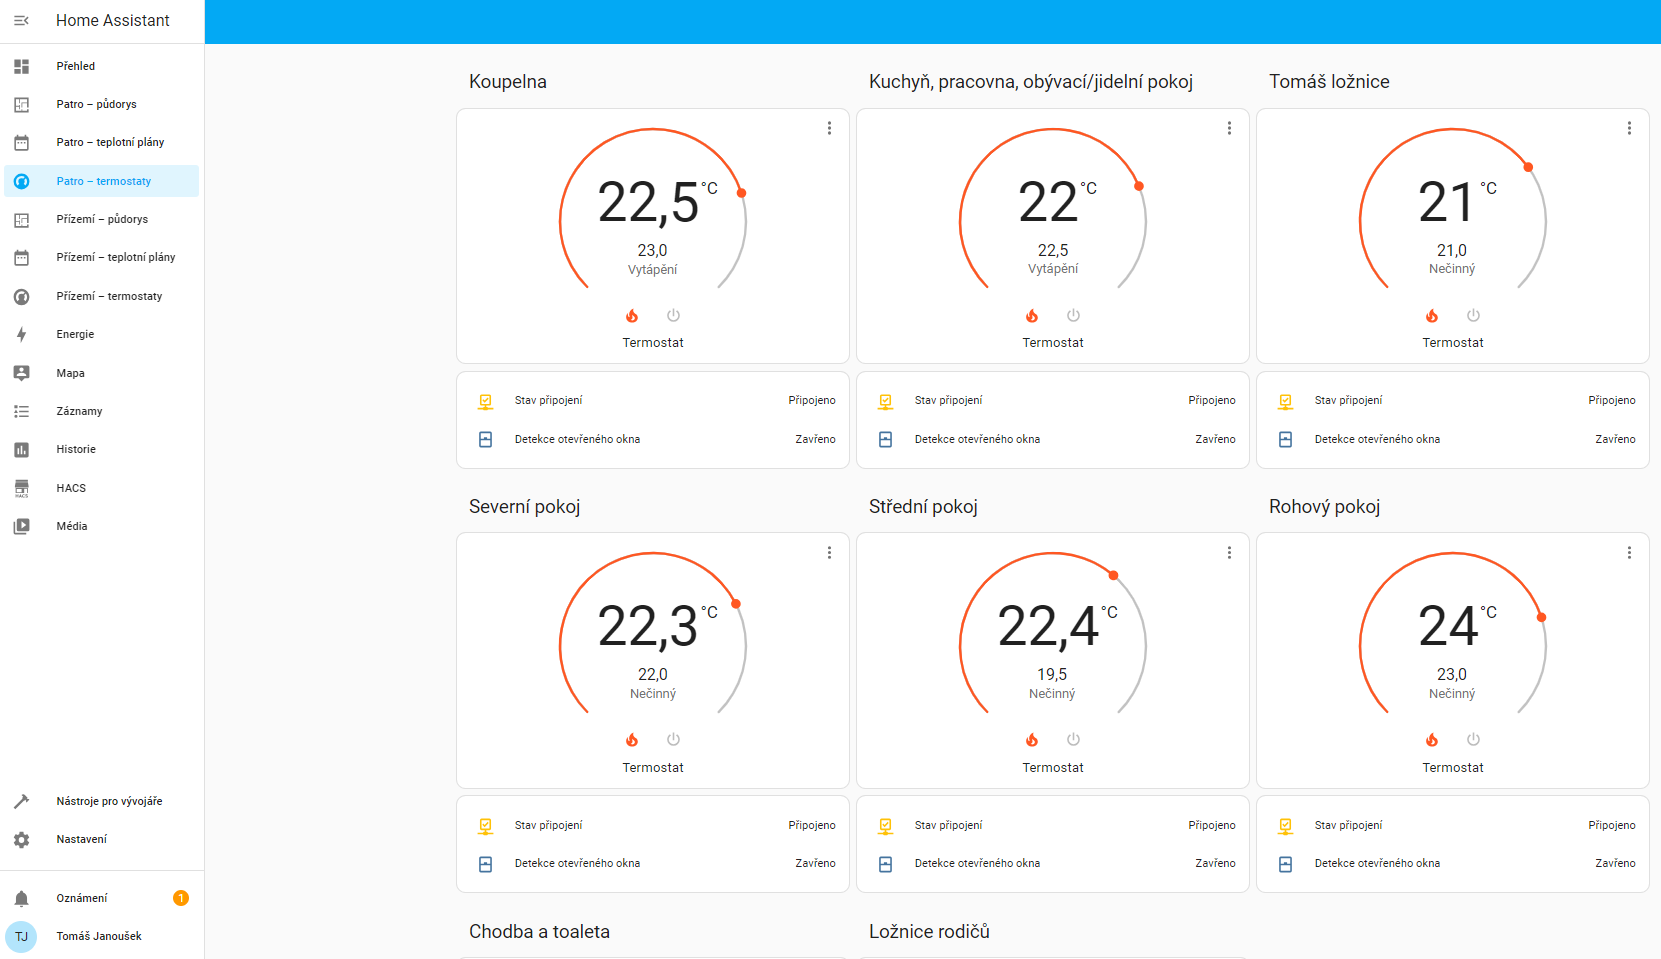
\includegraphics[width=1\textwidth]{pictures/czech/software/thermostats-first-floor.png}
    \caption{The First Floor – Thermostats.}
    \label{fig:thermostats-first-floor}
\end{figure}
\end{English}

\begin{Czech}
\begin{figure}[H]
    \centering
    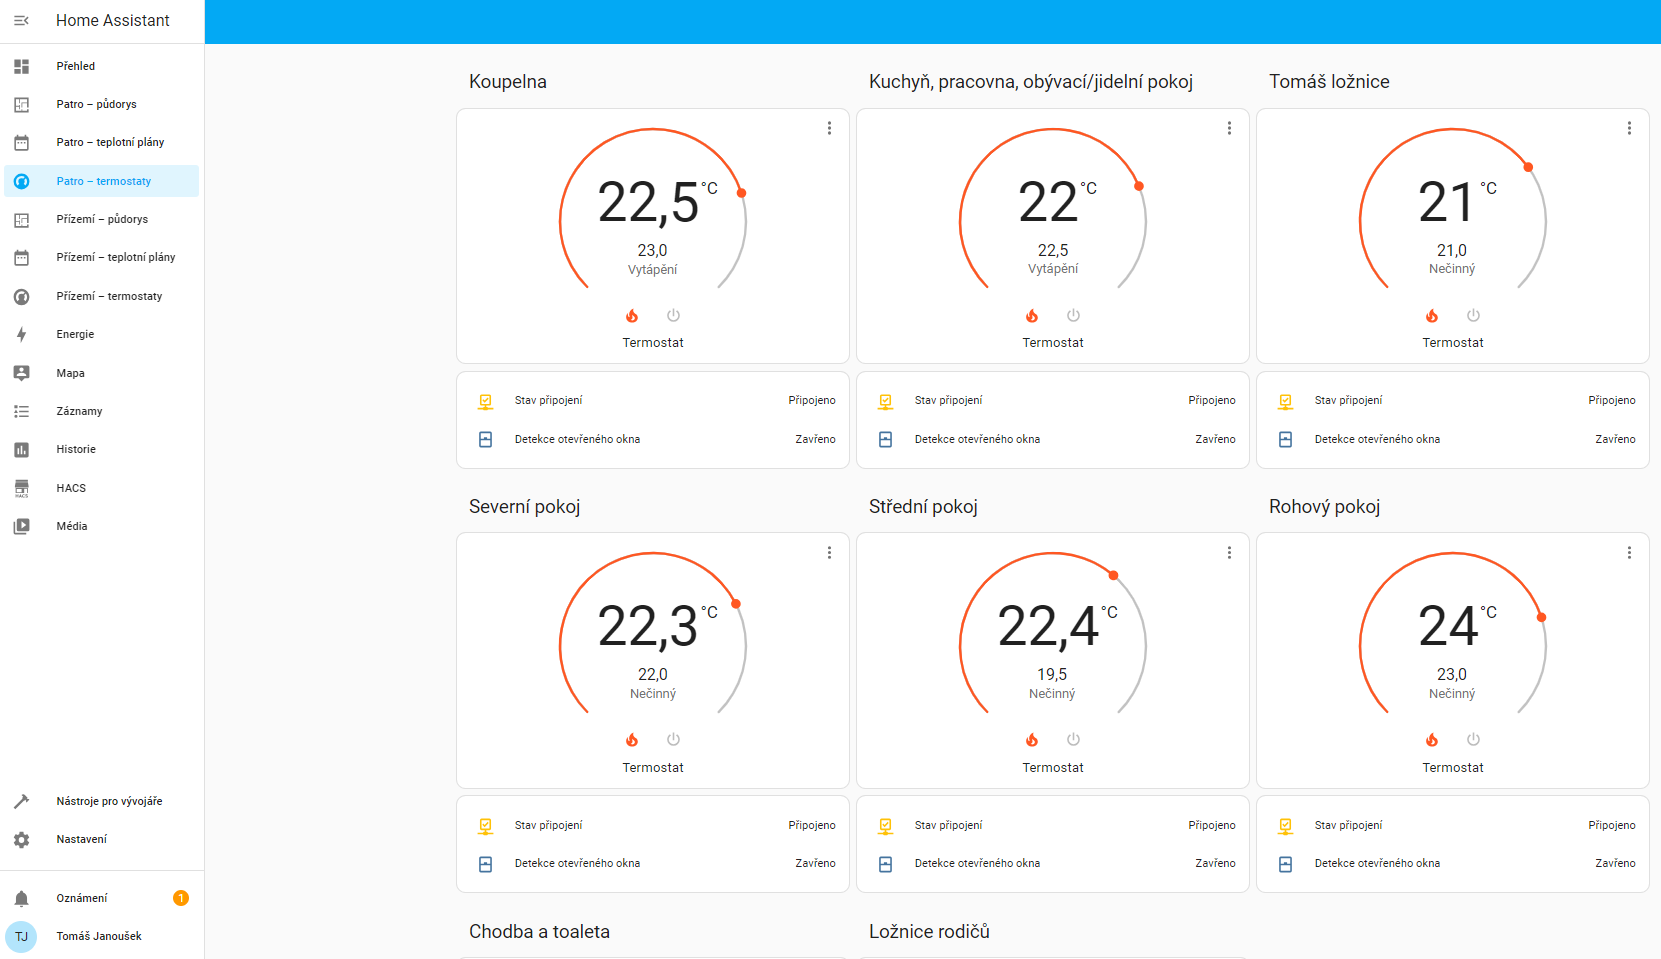
\includegraphics[width=1\textwidth]{pictures/czech/software/thermostats-first-floor.png}
    \caption{Patro – termostaty.}
    \label{fig:thermostats-first-floor}
\end{figure}
\end{Czech}


\begin{English}
\begin{figure}[H]
    \centering
    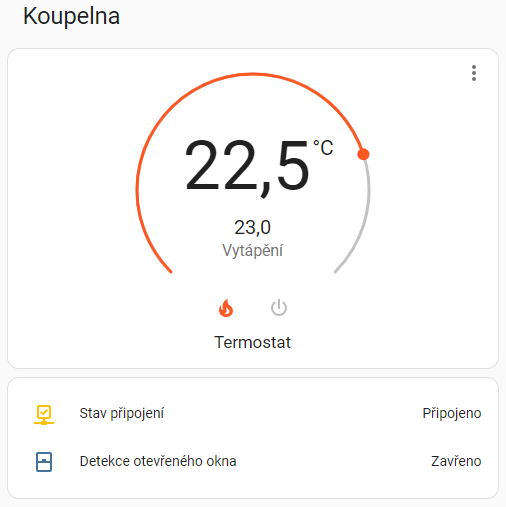
\includegraphics[width=0.5\textwidth]{pictures/czech/software/thermostat.png}
    \caption{Thermostat – Bathroom.}
    \label{fig:thermostat}
\end{figure}
\end{English}

\begin{Czech}
\begin{figure}[H]
    \centering
    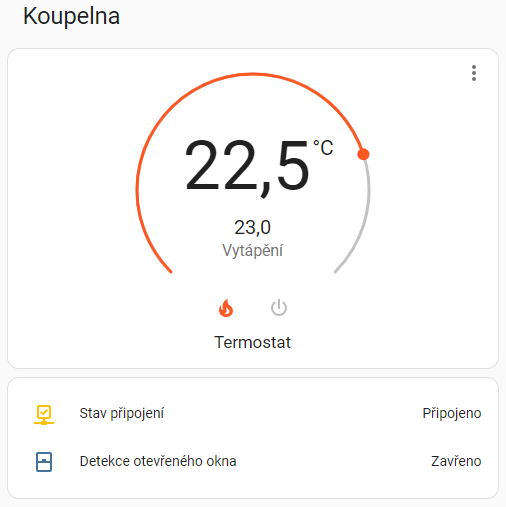
\includegraphics[width=0.5\textwidth]{pictures/czech/software/thermostat.png}
    \caption{Termostat – koupelna.}
    \label{fig:thermostat}
\end{figure}
\end{Czech}


\begin{English}
\begin{figure}[H]
    \centering
    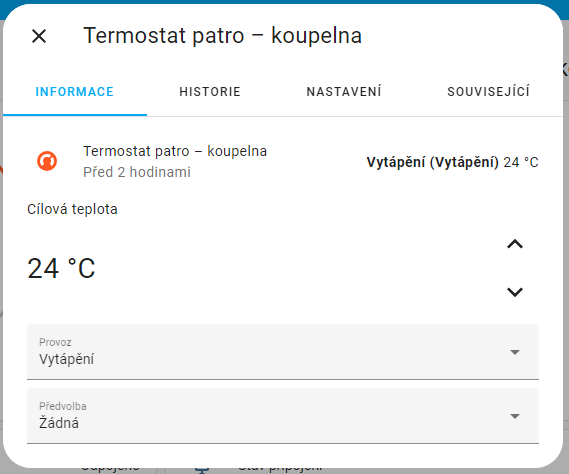
\includegraphics[width=0.5\textwidth]{pictures/czech/software/click-thermostat.png}
    \caption{Clicking on 3 dots in the top right corner of thermostat – bathroom.}
    \label{fig:click-thermostat}
\end{figure}
\end{English}

\begin{Czech}
\begin{figure}[H]
    \centering
    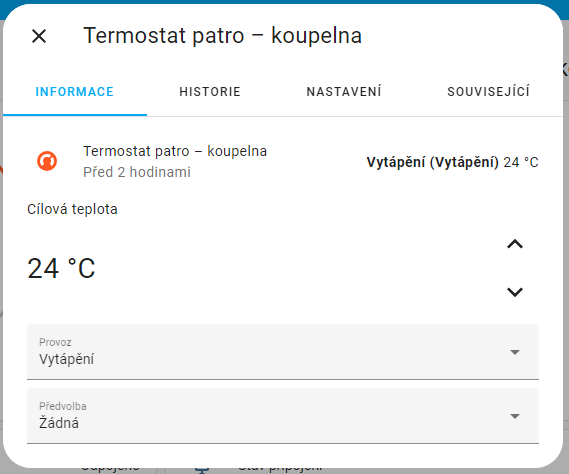
\includegraphics[width=0.5\textwidth]{pictures/czech/software/click-thermostat.png}
    \caption{Kliknutí na 3 tečky v pravém horním rohu termostatu – koupelna.}
    \label{fig:click-thermostat}
\end{figure}
\end{Czech}

% ========================================

\begin{English}
\subsubsubsection{Automatic Control According to Temperature Plans}
\end{English}

\begin{Czech}
\subsubsubsection{Automatické řízení podle teplotních plánů}
\end{Czech}


\begin{English}
In mode "\textit{Automatic Control According to Temperature Plans}" is control of heating according to wall temperature sensor for each room. However, it takes place on the basis of temperature plans, setting the desired temperature (the figure \ref{fig:temperature-plan-ground-floor}).
\end{English}

\begin{Czech}
V módu „\textit{Automatické řízení podle teplotních plánů}“ docházení k řízení vytápění podle nástěnných snímačů teploty pro každou místnost. Dochází však na základě teplotních plánů nastavování požadované teploty (obrázek \ref{fig:temperature-plan-ground-floor}).
\end{Czech}


\begin{English}
\begin{figure}[H]
    \centering
    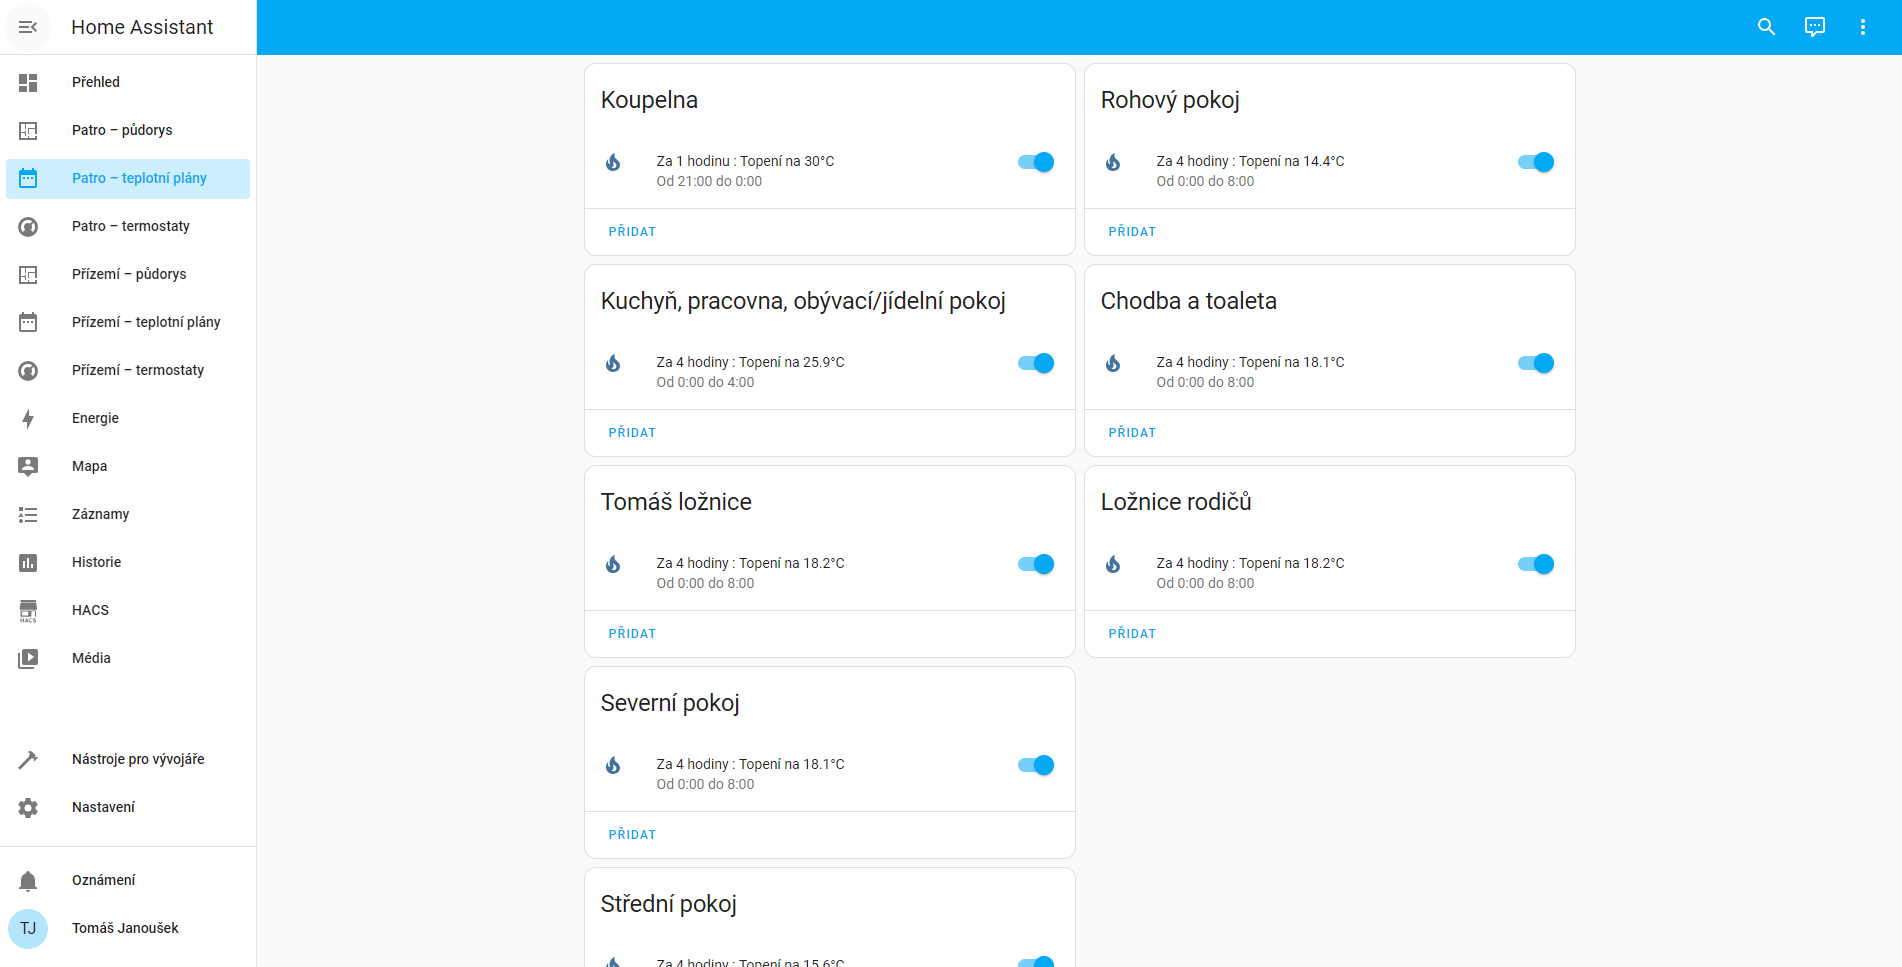
\includegraphics[width=1\textwidth]{pictures/czech/software/temperature-plan-ground-floor.png}
    \caption{Temperature Plans for Control.}
    \label{fig:temperature-plan-ground-floor}
\end{figure}
\end{English}

\begin{Czech}
\begin{figure}[H]
    \centering
    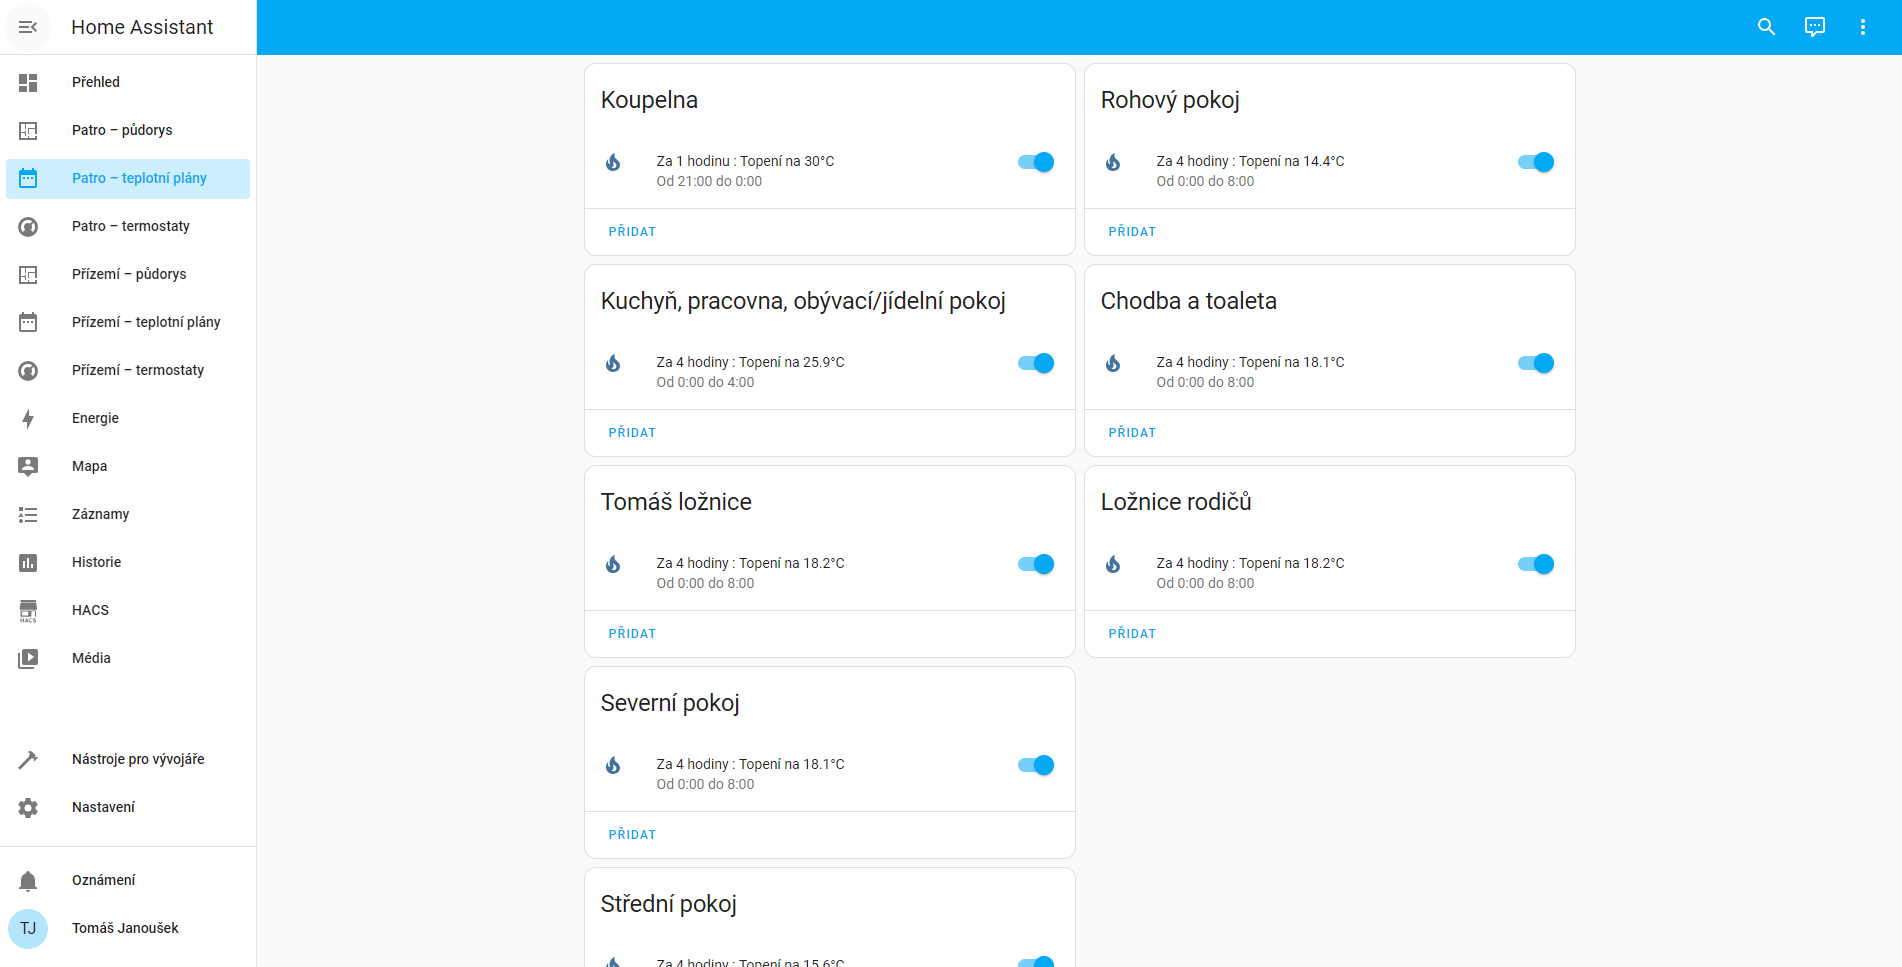
\includegraphics[width=1\textwidth]{pictures/czech/software/temperature-plan-ground-floor.png}
    \caption{Teplotní plány pro přízení.}
    \label{fig:temperature-plan-ground-floor}
\end{figure}
\end{Czech}


\begin{English}
There is a predefined temperature plan for each room. To make adjustments, simply click on it and the figure \ref{fig:temperature-plan-thermostat} will appear. To modify the temperature of a specific section, click on the desired section and use the slider below to change the temperature. Alternatively, you can add or delete a section. Then, save the settings using the buttons at the bottom right. Based on this configured temperature plan, the desired temperature for the room's thermostat is set, which controls the heating of that room.
\end{English}

\begin{Czech}
Pro každou místnost je předdefinovaný teplotní plán. Pro úpravu stačí na něho kliknout, zobrazí se obrázek \ref{fig:temperature-plan-thermostat}. Pro úpravu teploty daného úseku stačí kliknout na vybraný úsek a pomocí posuvníku dole změnit teplotu. Případně je možné daný úsek přidat nebo smazat. Následně dané nastavení uložit tlačítek vpravo dole. Na základě takto nastaveného teplotního plánu dochází k nastavení požadované teplotu to nástěnného snímače podle kterého se řídí  vytápění dané místnosti.
\end{Czech}


\begin{English}
\begin{figure}[H]
    \centering
    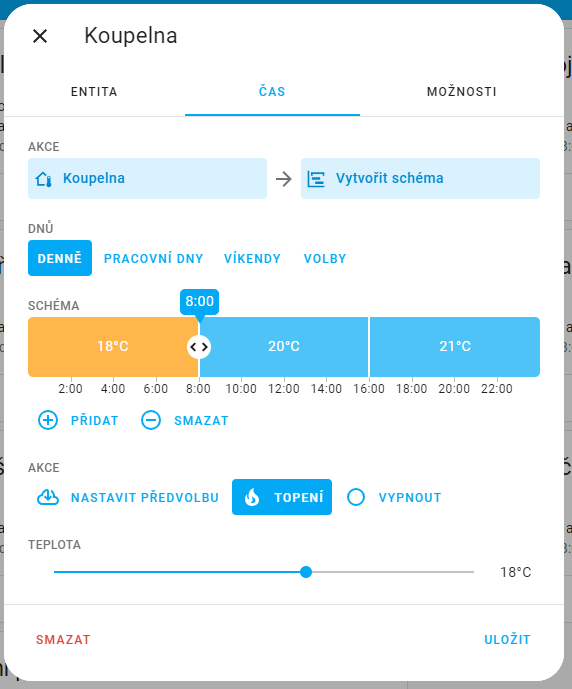
\includegraphics[width=0.5\textwidth]{pictures/czech/software/temperature-plan-thermostat.png}
    \caption{Settings/adjustment of the temperature plan.}
    \label{fig:temperature-plan-thermostat}
\end{figure}
\end{English}

\begin{Czech}
\begin{figure}[H]
    \centering
    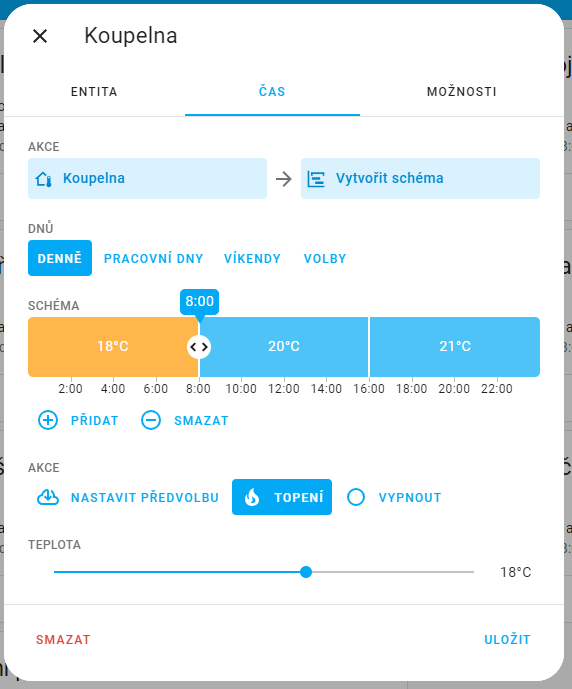
\includegraphics[width=0.5\textwidth]{pictures/czech/software/temperature-plan-thermostat.png}
    \caption{Nastavení/úprava teplotního plánu.}
    \label{fig:temperature-plan-thermostat}
\end{figure}
\end{Czech}

% ========================================

\begin{English}
\subsubsection{Control Modes}
\end{English}

\begin{Czech}
\subsubsection{Módy řízení}
\end{Czech}
\label{sec:control-modes}


\begin{English}
Based on the selected control modes (the figure \ref{fig:control-modes}), the heating coil in the hot water tank ir regulated. The limit of the min. top sensor and the max. middle sensor are determined according to chosen summer or winter mode (the figure \ref{fig:switching-heating-coil}). Control diagram  for the specified mode is shown in the figure \ref{fig:diagram-control-modes}.´
\end{English}

\begin{Czech}
Na základě zvoleného módu řízení (obrázek \ref{fig:control-modes}) dojde k řízení topné spirály v zásobníku otopné vody. Meze min. horní čidlo a max. střední čidlo se berou podle vybrané letního nebo zimního módu (obrázek \ref{fig:switching-heating-coil}). Diagram řízení pro daný mód je na obrázku \ref{fig:diagram-control-modes}.
\end{Czech}


\begin{English}
\begin{figure}[H]
    \centering
    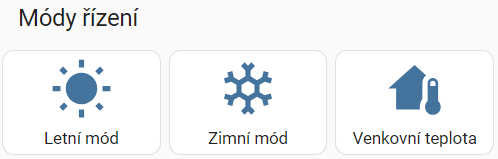
\includegraphics[width=0.7\textwidth]{pictures/czech/software/control-modes.png}
    \caption{Control Modes.}
    \label{fig:control-modes}
\end{figure}
\end{English}

\begin{Czech}
\begin{figure}[H]
    \centering
    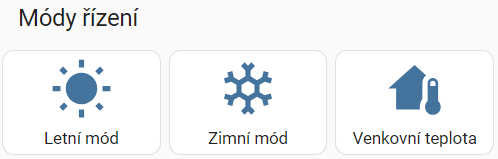
\includegraphics[width=0.7\textwidth]{pictures/czech/software/control-modes.png}
    \caption{Módy řízení.}
    \label{fig:control-modes}
\end{figure}
\end{Czech}


\begin{English}
\begin{figure}[H]
    \centering
    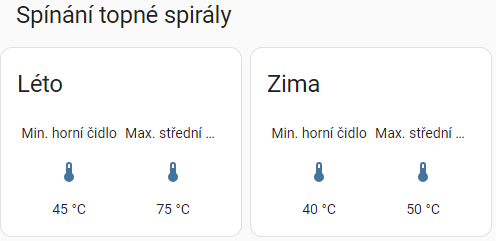
\includegraphics[width=0.7\textwidth]{pictures/czech/software/switching-heating-coil.png}
    \caption{Switching of Heating Coil.}
    \label{fig:switching-heating-coil}
\end{figure}
\end{English}

\begin{Czech}
\begin{figure}[H]
    \centering
    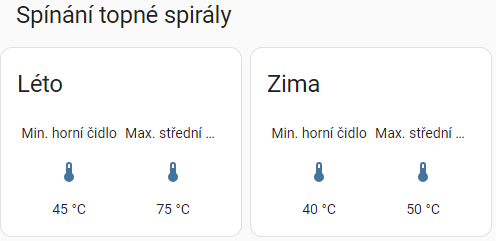
\includegraphics[width=0.7\textwidth]{pictures/czech/software/switching-heating-coil.png}
    \caption{Spínání topné spirály.}
    \label{fig:switching-heating-coil}
\end{figure}
\end{Czech}


\begin{English}
\begin{figure}[H]
    \centering
    \def\svgwidth{1\columnwidth}
    \graphicspath{{pictures/czech/software/svg/}}
    \input{pictures/czech/software/svg/diagram-control-modes.pdf_tex}
    \caption{Control diagram mode.}
    \label{fig:diagram-control-modes}
\end{figure}
\end{English}

\begin{Czech}
\begin{figure}[H]
    \centering
    \def\svgwidth{1\columnwidth}
    \graphicspath{{pictures/czech/software/svg/}}
    \input{pictures/czech/software/svg/diagram-control-modes.pdf_tex}
    \caption{Diagram módu řízení.}
    \label{fig:diagram-control-modes}
\end{figure}
\end{Czech}

% ========================================

\begin{English}
\subsubsubsection{Other Settings}
\end{English}

\begin{Czech}
\subsubsubsection{Ostatní nastavení}
\end{Czech}


\begin{English}
In the section "\textit{Other Settings}" it is possible to set the hysteresis of heating coil which is used in \textbf{Control Modes}. In the section "\textit{Min. Outdoor Temperature for Summer Mode}" is defined a threshold to determine whether it is a summer or winter mode. If the outdoor temperature is greater than or equal to this threshold,  he summer mode is selected otherwise the winter mode is chosen.
\end{English}

\begin{Czech}
V části „\textit{ostatní nastavení}“ je možné nastavit hysterezi spirály využívanou v \textbf{módech řízení}. V „\textit{Min. venkovní teplota pro letní mód}“ se definuje mez pro určení, zda se jedná o letní nebo zimní mód. Pokud je venkovní teplota vetší nebo rovna této mezi zvolí se letní mód jinak zimní.
\end{Czech}


\begin{English}
\begin{figure}[H]
    \centering
    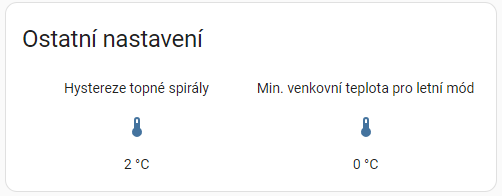
\includegraphics[width=0.7\textwidth]{pictures/czech/software/other-settings.png}
    \caption{Other Settings.}
    \label{fig:other-settings}
\end{figure}
\end{English}

\begin{Czech}
\begin{figure}[H]
    \centering
    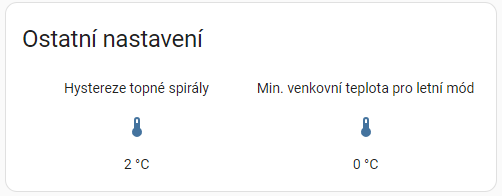
\includegraphics[width=0.7\textwidth]{pictures/czech/software/other-settings.png}
    \caption{Ostatní nastavení.}
    \label{fig:other-settings}
\end{figure}
\end{Czech}

% ========================================

\begin{English}
\subsubsection{Fireplaces – Switching of Pumps}
\end{English}

\begin{Czech}
\subsubsection{Krby – spínání čerpadel}
\end{Czech}


\begin{English}
In the figure \ref{fig:diagram-fireplace}, there is the diagram to turn on circulation pumps for fireplaces in case of flooding. This settings is the same for all fireplace pumps, only the min. threshold for activation differs  (the figure \ref{fig:fireplace-switching-pumps}).
\end{English}

\begin{Czech}
Na obrázku \ref{fig:diagram-fireplace} je diagram pro sepnutí oběhových čerpadel pro krby v případě zatopení. Pro všechny krbová čerpadla je toto nastavení stejné, liší se pouze min. mez pro sepnutí (obrázek\ref{fig:fireplace-switching-pumps}).
\end{Czech}


\begin{English}
\begin{figure}[H]
    \centering
    \def\svgwidth{1\columnwidth}
    \graphicspath{{pictures/czech/software/svg/}}
    \input{pictures/czech/software/svg/diagram-fireplace.pdf_tex}
    \caption[]{Diagram to turn on circulation pumps for fireplaces.}
    \label{fig:diagram-fireplace}
\end{figure}
\end{English}

\begin{Czech}
\begin{figure}[H]
    \centering
    \def\svgwidth{1\columnwidth}
    \graphicspath{{pictures/czech/software/svg/}}
    \input{pictures/czech/software/svg/diagram-fireplace.pdf_tex}
    \caption[]{Diagram sepnutí oběhových čerpadel pro krby.}
    \label{fig:diagram-fireplace}
\end{figure}
\end{Czech}


\begin{English}
\begin{figure}[H]
    \centering
    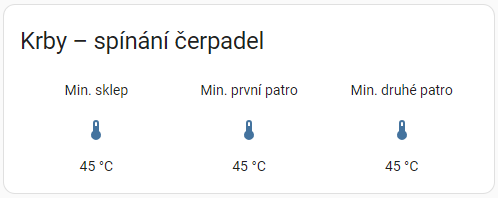
\includegraphics[width=0.7\textwidth]{pictures/czech/software/fireplace-switching-pumps.png}
    \caption{Settings min. threshold for turn on circulation pumps for fireplaces in case flood.}
    \label{fig:fireplace-switching-pumps}
\end{figure}
\end{English}

\begin{Czech}
\begin{figure}[H]
    \centering
    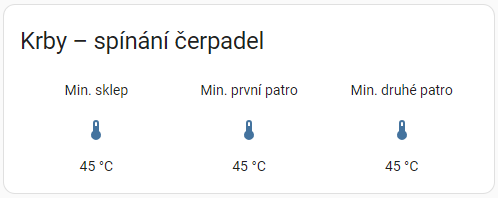
\includegraphics[width=0.7\textwidth]{pictures/czech/software/fireplace-switching-pumps.png}
    \caption{Nastavení min. mezí pro sepnutí oběhových čerpadel pro krby v případě zatopení.}
    \label{fig:fireplace-switching-pumps}
\end{figure}
\end{Czech}


\begin{English}
\tipbox{Note}{This setting is completely independent of other system settings. In case of flooding, the pump must always be activated.}
\end{English}

\begin{Czech}
\tipbox{Poznámka}{Toto nastavení je zcela nezávislé na dalších nastavení systému. \mbox{V případě} zatopení musí dojít vždy \mbox{k sepnutí} čerpadla.}
\end{Czech}

% ========================================

\begin{English}
\subsubsection{The LED Indication – limiting parameters of the hot water tank}
\end{English}

\begin{Czech}
\subsubsection{LED indikace – mezní parametry zásobníku teplé vody}
\end{Czech}
\label{sec:led-indication}


\begin{English}
In the picture \ref{fig:led-indication} are adjustable thresholds for controlling signaling LEDs for the hot water tank. Each LED indicates the heating or cooling section of the hot water tank. The red LED is for the bottom part, the orange LED for the middle part and the blue LED for the top part of hot water tank. In case the temperature in the bottom or middle part is greater than the thresholds set for the red or orange LED, the red or orange LED will light up. In case the temperature in top part is lower than the threshold for blue LED, the blue LED will light up. The diagram is for red respectively orange LED is in the figure \ref{fig:diagram-red-orange-led-indication}. The diagram for the blue LED is in the figure \ref{fig:diagram-blue-led-indication}.
\end{English}

\begin{Czech}
Na obrázku \ref{fig:led-indication} jsou nastavitelné meze pro ovládání signalizačních LED pro zásobník otopné vody. Jednotlivé LED označují natopení respektive chladnou část zásobníku otopné vody. Červená LED je pro spodní část, oranžová LED pro střední část a modrá LED pro horní část zásobníku otopné vody. V případě, že teplota ve spodní respektive střední části je větší než meze nastavené pro červenou respektive oranžovou LED, dojde k rozsvícení červené respektive oranžové LED. V případě, že teplota v horní části je nižší než mez pro modrou LED, dojde k rozsvícení modré LED. Diagram pro červenou respektive oranžovou LED je na obrázku \ref{fig:diagram-red-orange-led-indication}. Diagram pro modrou LED je na obrázku \ref{fig:diagram-blue-led-indication}.
\end{Czech}


\begin{English}
\begin{figure}[H]
    \centering
    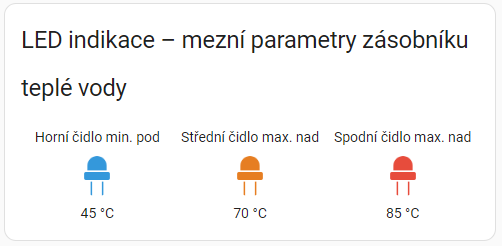
\includegraphics[width=0.65\textwidth]{pictures/czech/software/led-indication.png}
    \caption{Thresholds for controlling of signaling LED for the hot water tank.}
    \label{fig:led-indication}
\end{figure}
\end{English}

\begin{Czech}
\begin{figure}[H]
    \centering
    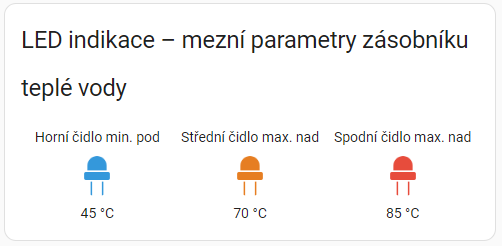
\includegraphics[width=0.65\textwidth]{pictures/czech/software/led-indication.png}
    \caption{Meze pro ovládání signalizační LED pro zásobník otopné vody.}
    \label{fig:led-indication}
\end{figure}
\end{Czech}


\begin{English}
\begin{figure}[H]
    \centering
    \def\svgwidth{1\columnwidth}
    \graphicspath{{pictures/czech/software/svg/}}
    \input{pictures/czech/software/svg/diagram-red-orange-led-indication.pdf_tex}
    \caption{The diagram for controlling red and orange signaling LED.}
    \label{fig:diagram-red-orange-led-indication}
\end{figure}
\end{English}

\begin{Czech}
\begin{figure}[H]
    \centering
    \def\svgwidth{1\columnwidth}
    \graphicspath{{pictures/czech/software/svg/}}
    \input{pictures/czech/software/svg/diagram-red-orange-led-indication.pdf_tex}
    \caption{Diagram ovládání červené a oranžové signalizační LED.}
    \label{fig:diagram-red-orange-led-indication}
\end{figure}
\end{Czech}


\begin{English}
\begin{figure}[H]
    \centering
    \def\svgwidth{1\columnwidth}
    \graphicspath{{pictures/czech/software/svg/}}
    \input{pictures/czech/software/svg/diagram-blue-led-indication.pdf_tex}
    \caption{The diagram for controlling blue signaling LED.}
    \label{fig:diagram-blue-led-indication}
\end{figure}
\end{English}

\begin{Czech}
\begin{figure}[H]
    \centering
    \def\svgwidth{1\columnwidth}
    \graphicspath{{pictures/czech/software/svg/}}
    \input{pictures/czech/software/svg/diagram-blue-led-indication.pdf_tex}
    \caption{Diagram ovládání modré signalizační LED.}
    \label{fig:diagram-blue-led-indication}
\end{figure}
\end{Czech}


\begin{English}
\tipbox{Note}{This settings is completely independent of other system settings.}
\end{English}

\begin{Czech}
\tipbox{Poznámka}{Toto nastavení je zcela nezávislé na dalších nastavení systému.}
\end{Czech}

% ====================  STOP Settings Tab ====================

% ====================  START Devices Tab ====================
\begin{English}
\subsection{Devices Tab}
\end{English}

\begin{Czech}
\subsection{Záložka zařízení}
\end{Czech}


\begin{English}
\subsubsection{End Devices}
\end{English}

\begin{Czech}
\subsubsection{Koncová zařízení}
\end{Czech}


\begin{English}
In the \textbf{devices} tab in the figure \ref{fig:tab-devices} (the top blue menu) are shown in the section "\textit{End Devices}". The state respectively option for turn on/off given device (the figure \ref{fig:end-devices}). If the user wants to change the device state, they must set the "\textit{Manual Device Control}" button to the enabled state (blue state of the button) then it is possible to manually control the device. If the user changes the device state without the option of  "\textit{Manual Device Control}", it may result in overwriting the user's device settings according to the system state. At the LED is possible to see the on/off state for manual control of the LED is not available. 
\end{English}

\begin{Czech}
V záložce \textbf{zařízení} obrázek \ref{fig:tab-devices} (horní modré menu) jsou vidět v části „\textit{Koncová zařízení}“ stav respektive možnost zapnout/vypnout dané zařízení, obrázek \ref{fig:end-devices}. V případě, že uživatel chce měnit stav zařízení musí uvést tlačítko „\textit{Manuální ovládání zařízení}“ do stavu zapnuto (modrý stav tlačítka), pak je možné manuálně ovládat zřízení. \mbox{V případě}, že uživatel změní stav zařízení bez možnosti „\textit{Manuální ovládání zařízení}“ může dojít k přepsaní uživatelského nastavení zařízení podle stavu ze systému. U LED je možné pouze vidět stav zapnuto/vypnuto manuální ovládání LED není k dipozici.
\end{Czech}


\begin{English}
\begin{figure}[H]
    \centering
    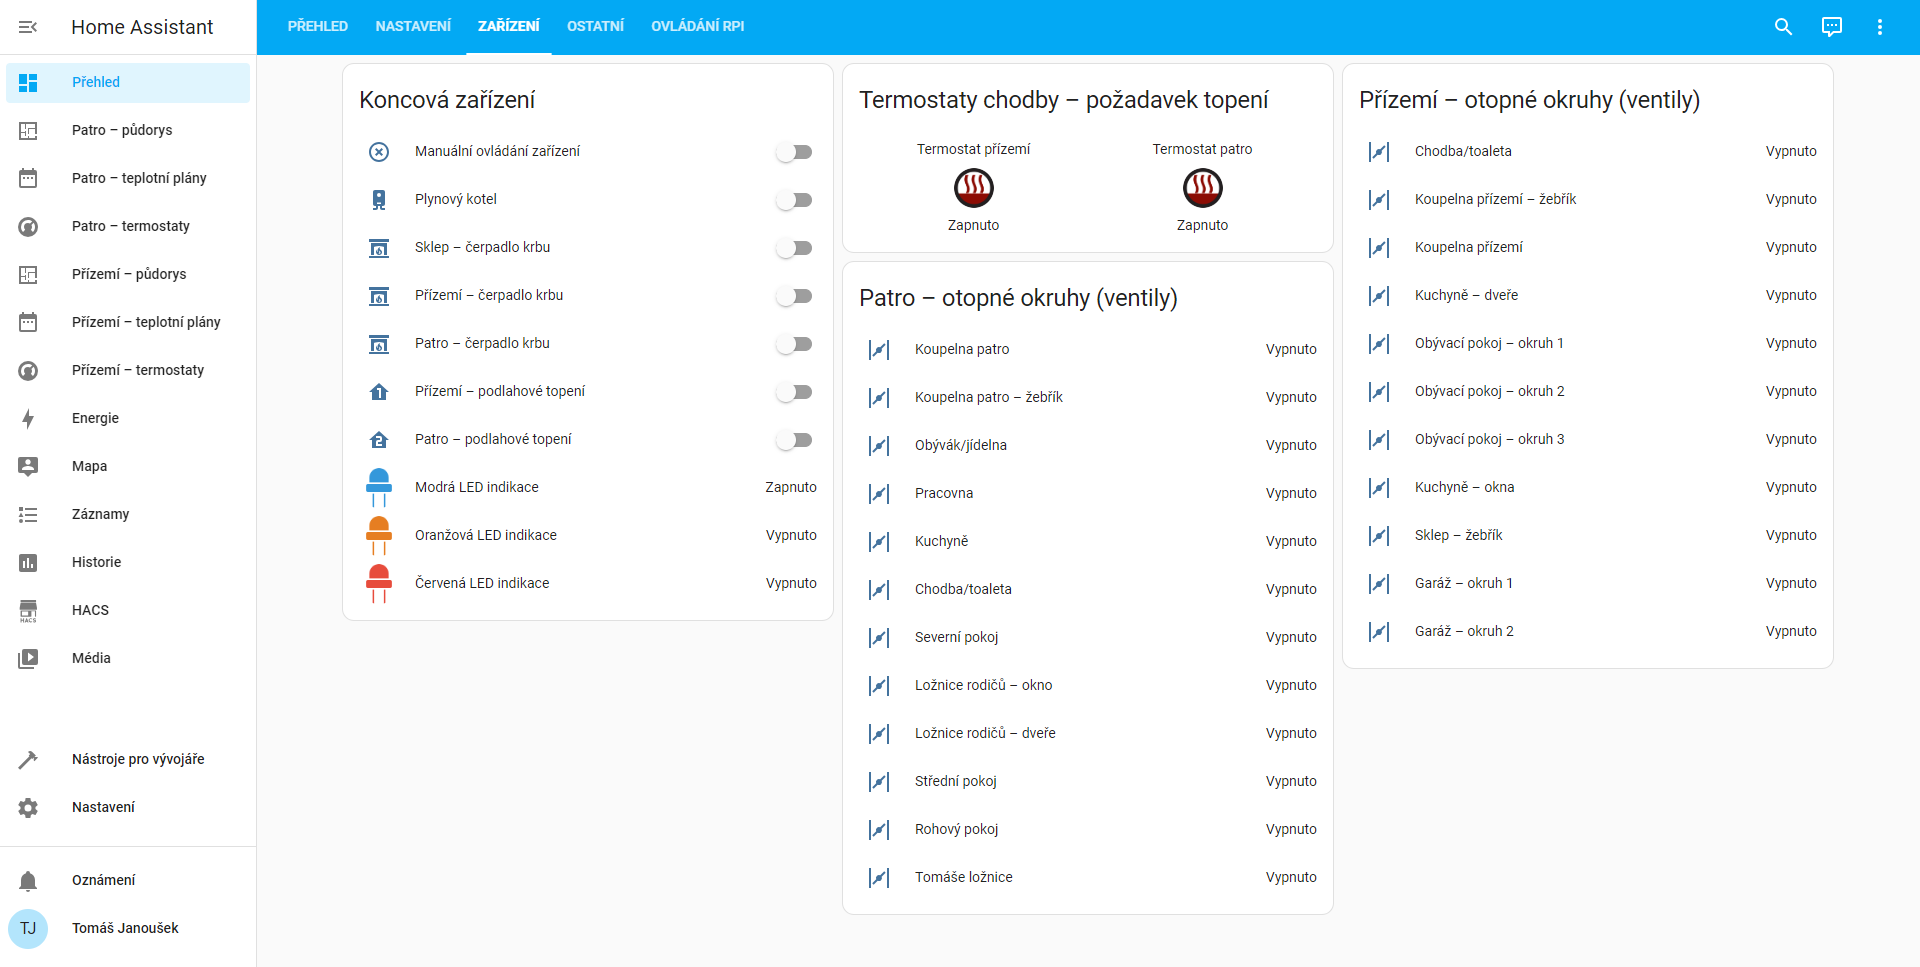
\includegraphics[width=1\textwidth]{pictures/czech/software/devices-tab.png}
    \caption{Devices Tab.}
    \label{fig:tab-devices}
\end{figure}
\end{English}

\begin{Czech}
\begin{figure}[H]
    \centering
    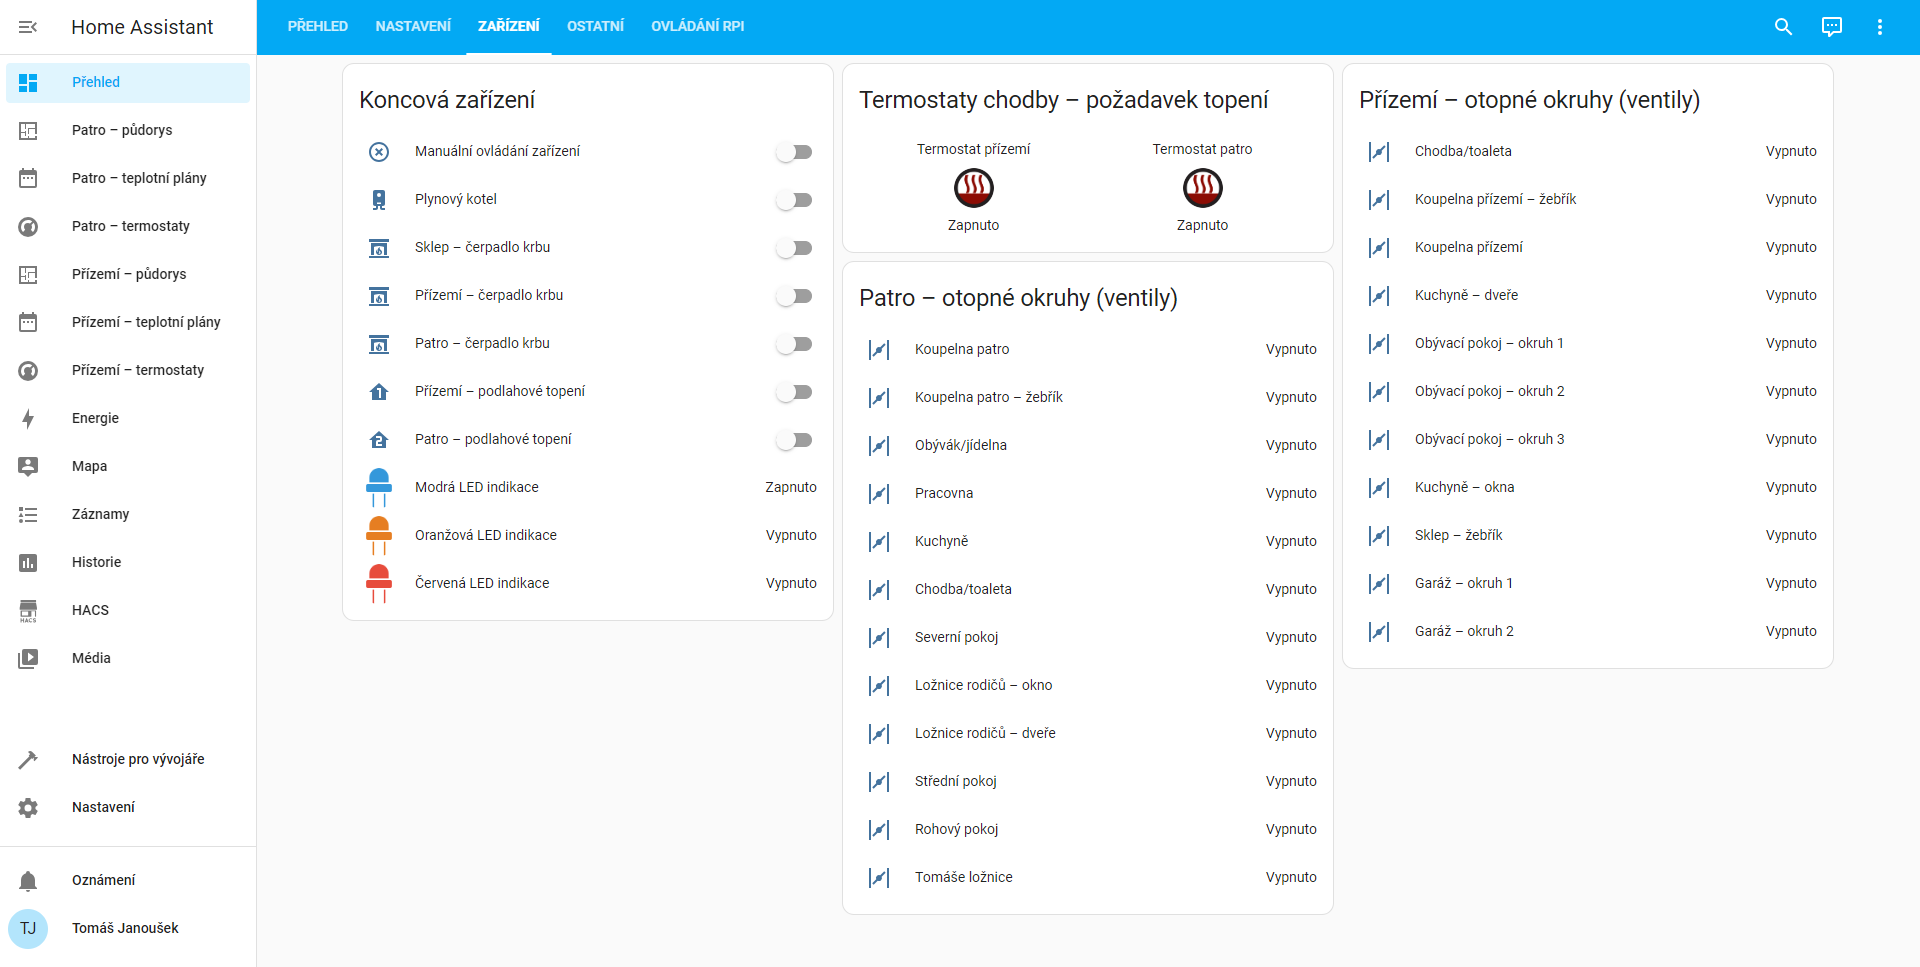
\includegraphics[width=1\textwidth]{pictures/czech/software/devices-tab.png}
    \caption{Záložka zařízení.}
    \label{fig:tab-devices}
\end{figure}
\end{Czech}


\begin{English}
\begin{figure}[H]
    \centering
    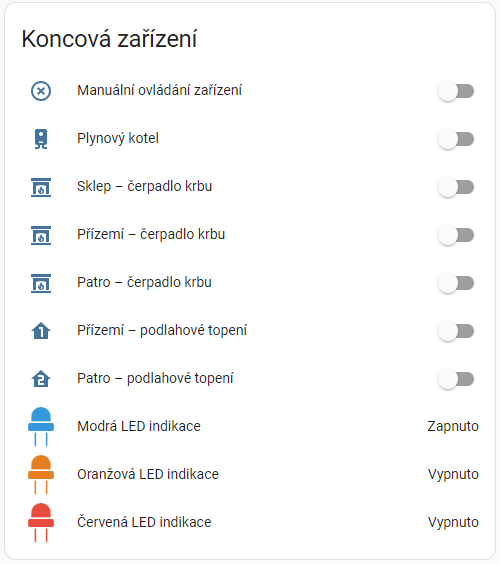
\includegraphics[width=0.6\textwidth]{pictures/czech/software/end-devices.png}
    \caption{End Devices.}
    \label{fig:end-devices}
\end{figure}
\end{English}

\begin{Czech}
\begin{figure}[H]
    \centering
    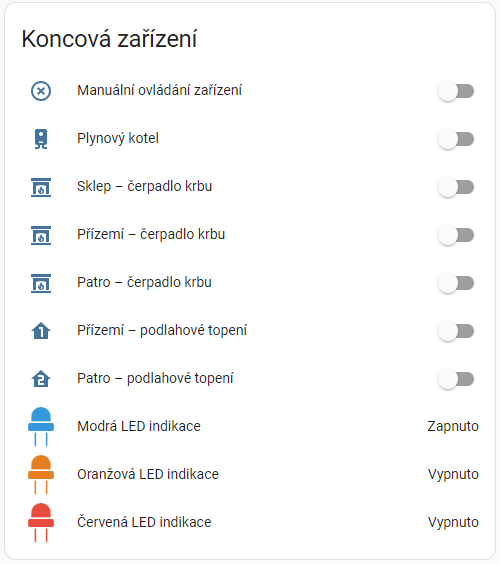
\includegraphics[width=0.6\textwidth]{pictures/czech/software/end-devices.png}
    \caption{Koncová zařízení.}
    \label{fig:end-devices}
\end{figure}
\end{Czech}


\begin{English}
\tipbox{Attention!!!}{If the user sets button "Manual Control Devices" to the enabled state. The system \textbf{can not} subsequently control the device according to the configured automation. It is necessary to always return the button to the \textbf{disabled} state.}
\end{English}

\begin{Czech}
\tipbox{Pozor!!!}{Pokud uživatel nastaví tlačítko „Manuální ovládání zařízení“ do stavu zapnuto. Systém \textbf{nemůže} následně zařízení ovládat podle nastavené automatizace. Je nutné vždy tlačítko vrátit do stavu \textbf{vypnuto}.}
\end{Czech}

% ========================================

\begin{English}
\subsubsection{Thermostats Corridors – Heating Requirement}
\end{English}

\begin{Czech}
\subsubsection{Termostaty chodby – požadavek topení}
\end{Czech}


\begin{English}
In the figure \ref{fig:corridor-thermostats2} is shown state on/off for corridor thermostat. This setting is further used in heating mode "Control Temperature from Corridor Thermostats", more information in the section "Control Temperature from Corridor Thermostats".
\end{English}

\begin{Czech}
Na obrázku \ref{fig:corridor-thermostats2} je vidět stav zapnuto/vypnuto pro chodbové termostaty. Toto nastavení se dále používá v módu vytápění „Řízení teploty z chodbových termostatů“, více informací v sekci „Řízení teploty z chodbových termostatů“.
\end{Czech}


\begin{English}
\begin{figure}[H]
    \centering
    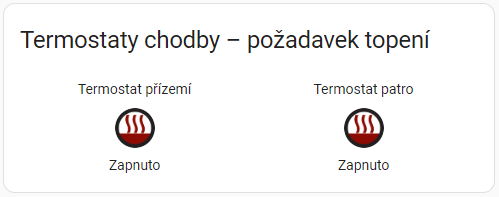
\includegraphics[width=0.6\textwidth]{pictures/czech/software/corridor-thermostats.png}
    \caption{Corridor Thermostats – Heating Requirement.}
    \label{fig:corridor-thermostats2}
\end{figure}
\end{English}

\begin{Czech}
\begin{figure}[H]
    \centering
    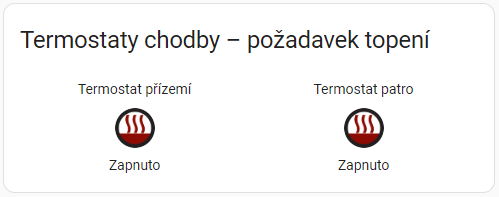
\includegraphics[width=0.6\textwidth]{pictures/czech/software/corridor-thermostats.png}
    \caption{Termostaty chodby – požadavek topení.}
    \label{fig:corridor-thermostats2}
\end{figure}
\end{Czech}

% ========================================

\begin{English}
\subsubsection{The Ground/First Floor – Heating Circuits (Valves)}
\end{English}

\begin{Czech}
\subsubsection{Přízemí/patro – otopné okruhy (ventily)}
\end{Czech}


\begin{English}
In the picture \ref{fig:heating-circuits-ground-floor2}  is shown state on/off valve for individual heating circuits, devied to the ground floor and the first floor. If the user  manual turns on valve with switch on the zone controller located na floor heating  distributors. The enabled state does not reflect in the system. The enabled state is not visible in the system. Manual activation via the switch should only be used if the system is non-functional. When the valve or heating circuit is manually turned on in this way, the corresponding circulation pump will be activated. The user doesn't have the option to manually turn on individual heating circuits through the system, only to view their status. Further information on controlling heating circuits is in the section \ref{sec:temperature-control} "\textit{Control Temperature}".
\end{English}

\begin{Czech}
Na obrázku \ref{fig:heating-circuits-ground-floor2} je vidět stav zapnuto/vypnuto ventilu pro jednotlivé otopné okruhy, rozdělené do přízemí a patra. Pokud uživatel manuálně zapne ventil přes vypínač na zónovém regulátoru umístěný na rozdělovačích podlahové vytápění. Stav zapnutí se nepromítne do systému, stav zapnuto není v systému vidět. Manuální zapnutí přes vypínač používat jen v případě, že systém je nefunkční. Při takto manuálním zapnutí ventilu respektive otopného okruhu dojde k sepnutí příslušného oběhového čerpadla. Uživatel nemá možnost manuálně přes systém zapínat jednotlivé otopné okruhy, pouze vidět jejich stav. Další informace o ovládání otopných okruhů je v části \ref{sec:temperature-control} „\textit{Řízení teploty}“.
\end{Czech}


\begin{English}
\begin{figure}[H]
    \centering
    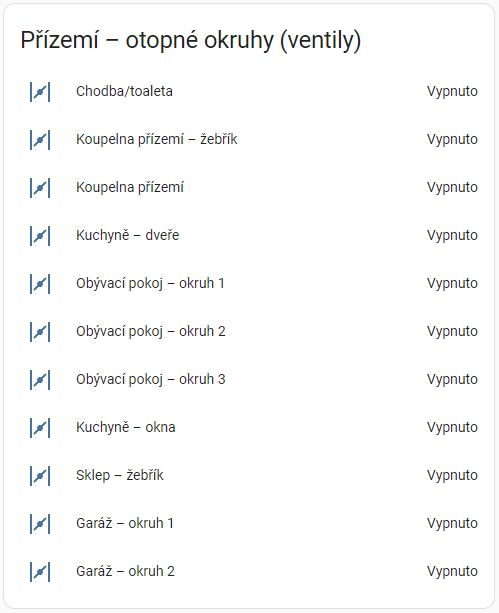
\includegraphics[width=0.6\textwidth]{pictures/czech/software/heating-circuits-ground-floor.png}
    \caption{The Ground Floor – Heating C11199ircuits (Valves).}
    \label{fig:heating-circuits-ground-floor2}
\end{figure}
\end{English}

\begin{Czech}
\begin{figure}[H]
    \centering
    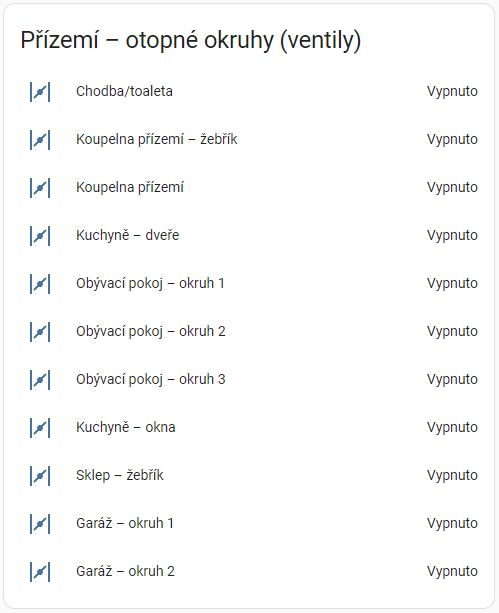
\includegraphics[width=0.6\textwidth]{pictures/czech/software/heating-circuits-ground-floor.png}
    \caption{Přízemí – otopné okruhy (ventily).}
    \label{fig:heating-circuits-ground-floor2}
\end{figure}
\end{Czech}

% ========================================

\newpage
\begin{English}
\subsection{Others Tab}
\end{English}

\begin{Czech}
\subsection{Záložka ostatní}
\end{Czech}


\begin{English}
In the \textbf{Others} tab, in the figure \ref{fig:tab-others} (the top blue menu) is shown setings for "\textit{Control of Pumps – Limescale}". This setting is useful for regular "flushing" of fireplace circulation pumps on a defined day and time with a specified duration of operation. If the pumps remain inactive for an extended period, they may become seized due to limescale buildup. This setting helps minimize this phenomenon by periodically running the pumps for a brief duration.
\end{English}

\begin{Czech}
V záložce \textbf{ostatní} obrázek \ref{fig:tab-others} (horní modré menu) je vidět nastavení pro „\textit{Ovládaní čerpadel – vodní kámen}“. Toto je nastavení je užitečné pro pravidelné „protočení“ krbových oběhový čerpadel v definovaný den a hodině s délkou spuštění. Pokud čerpadla delší dobu stojí, může dojít k zatuhnutí vlivem vodního kamene, toto nastavení tento jev minimalizuje. 
\end{Czech}


\begin{English}
\begin{figure}[H]
    \centering
    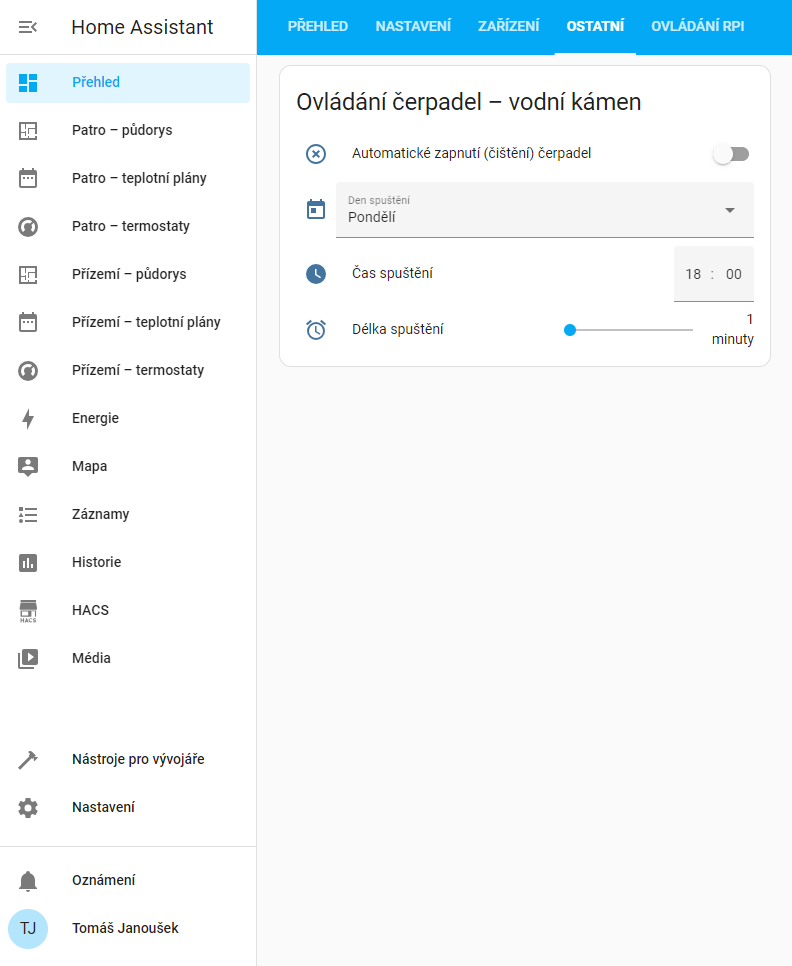
\includegraphics[width=0.6\textwidth]{pictures/czech/software/others-tab.png}
    \caption{Others Tab.}
    \label{fig:tab-others}
\end{figure}
\end{English}

\begin{Czech}
\begin{figure}[H]
    \centering
    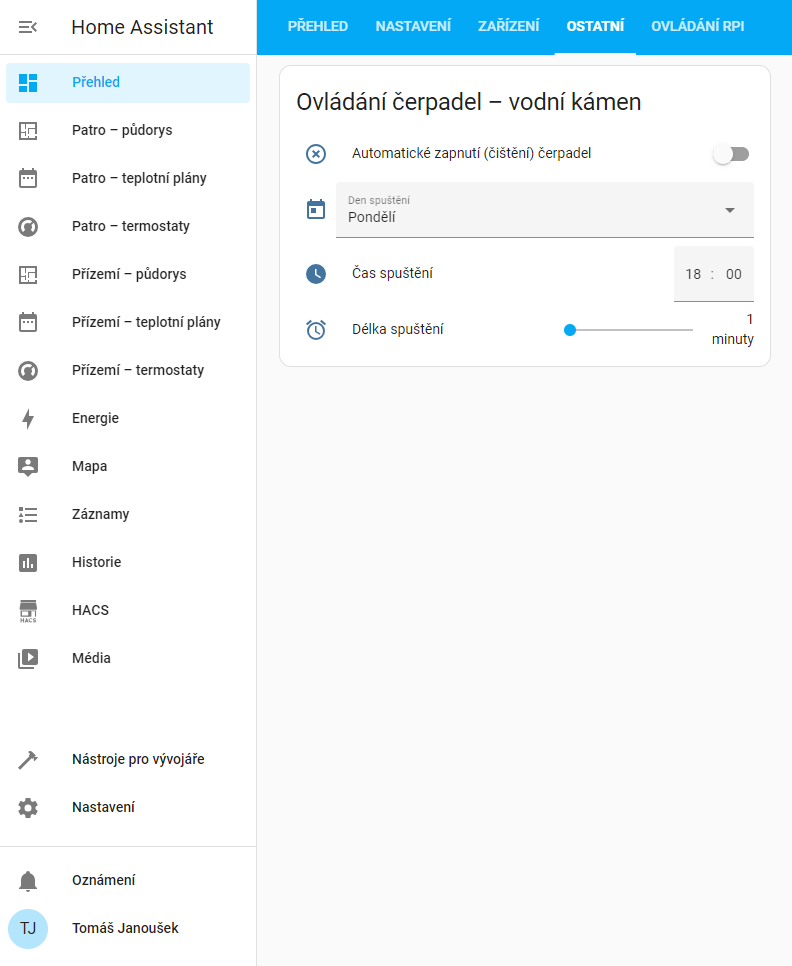
\includegraphics[width=0.6\textwidth]{pictures/czech/software/others-tab.png}
    \caption{Záložka ostatní.}
    \label{fig:tab-others}
\end{figure}
\end{Czech}

% ========================================

\newpage
\begin{English}
\subsection{The Ground/First Floor – The Ground Plan}
\end{English}

\begin{Czech}
\subsection{Přízemí/patro – půdorys}
\end{Czech}


\begin{English}
In \textbf{The Ground/First Floor – The Ground Plan} tab in the picture \ref{fig:floor-plan-first-floor} (the left menu) is shown the ground plan for the ground/first floor og house with individual currently measured temperatures, with desired temperatures, the heating status in the given room, and the status of the pumps or the heating status in the fireplace. After clicking on the desired temperature, it is possible to adjust the set temperature, etc. This setting is programmed into individual thermostats in the room.
\end{English}

\begin{Czech}
V záložce \textbf{Přízemí/patro – půdorys} obrázek \ref{fig:floor-plan-first-floor} (levé menu) je vidět půdorys pro přízemí/patro domu s jednotlivými aktuálně naměřenými teplotami, požadovanými teplotami, stavem topení v dané místnosti a stavem čerpadel respektive stavem topením v krbu. Po kliknutí na danou teplotu je možné měnit požadovanou teplotu apod. toto nastavení se propisuje do jednotlivých termostatů v místnosti.
\end{Czech}


\begin{English}
\begin{figure}[H]
    \centering
    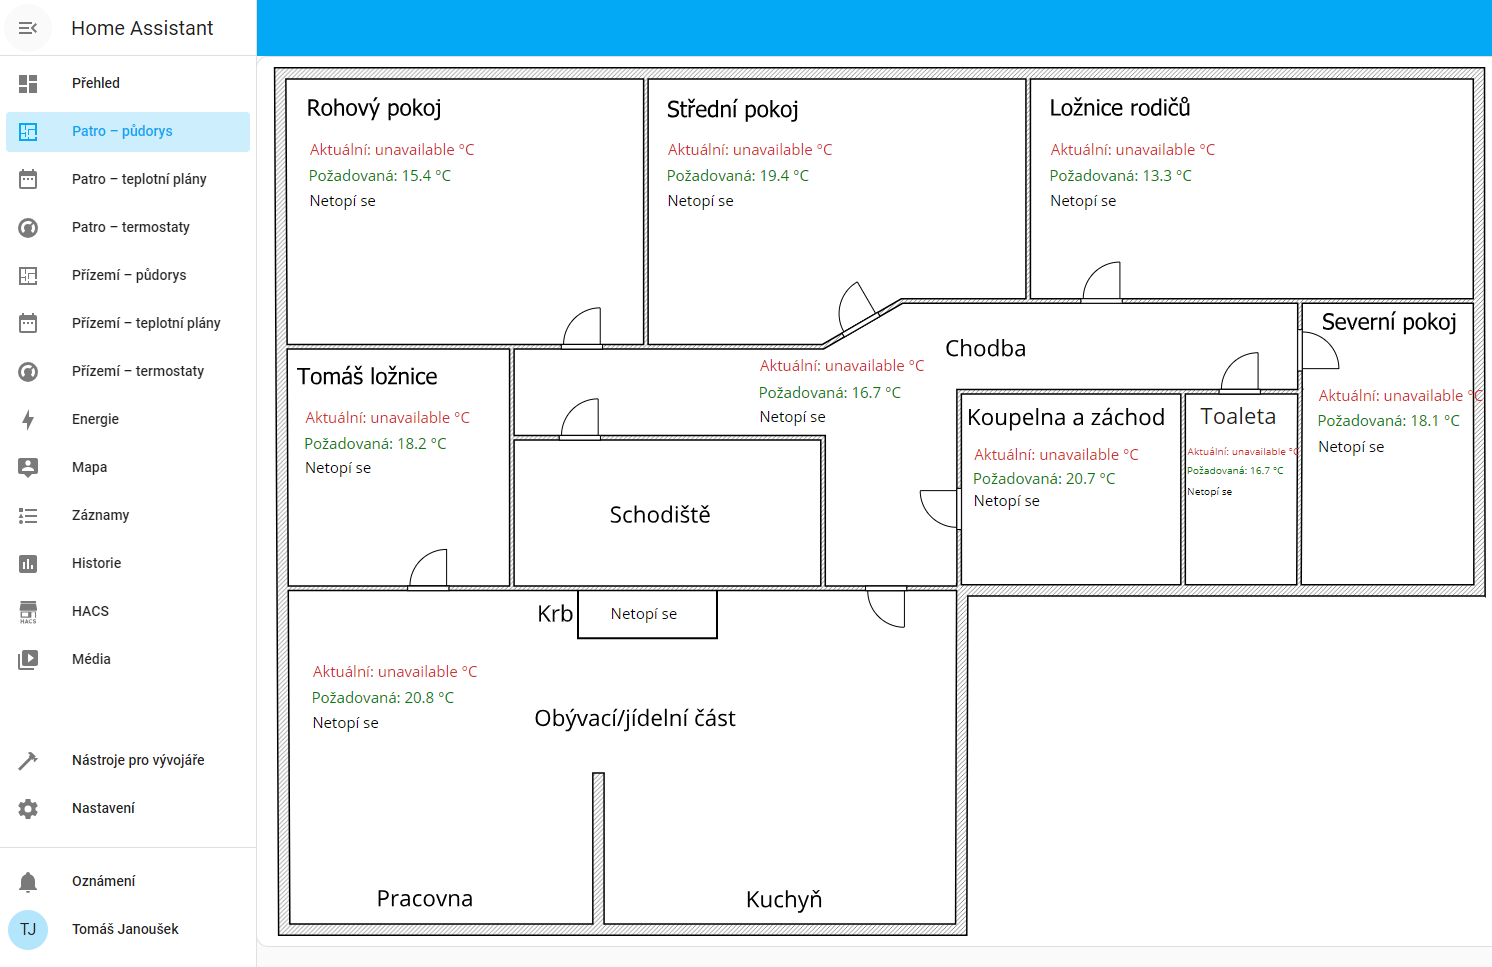
\includegraphics[width=1\textwidth]{pictures/czech/software/floor-plan-first-floor.png}
    \caption{The First Floor – The Ground Plan.}
    \label{fig:floor-plan-first-floor}
\end{figure}
\end{English}

\begin{Czech}
\begin{figure}[H]
    \centering
    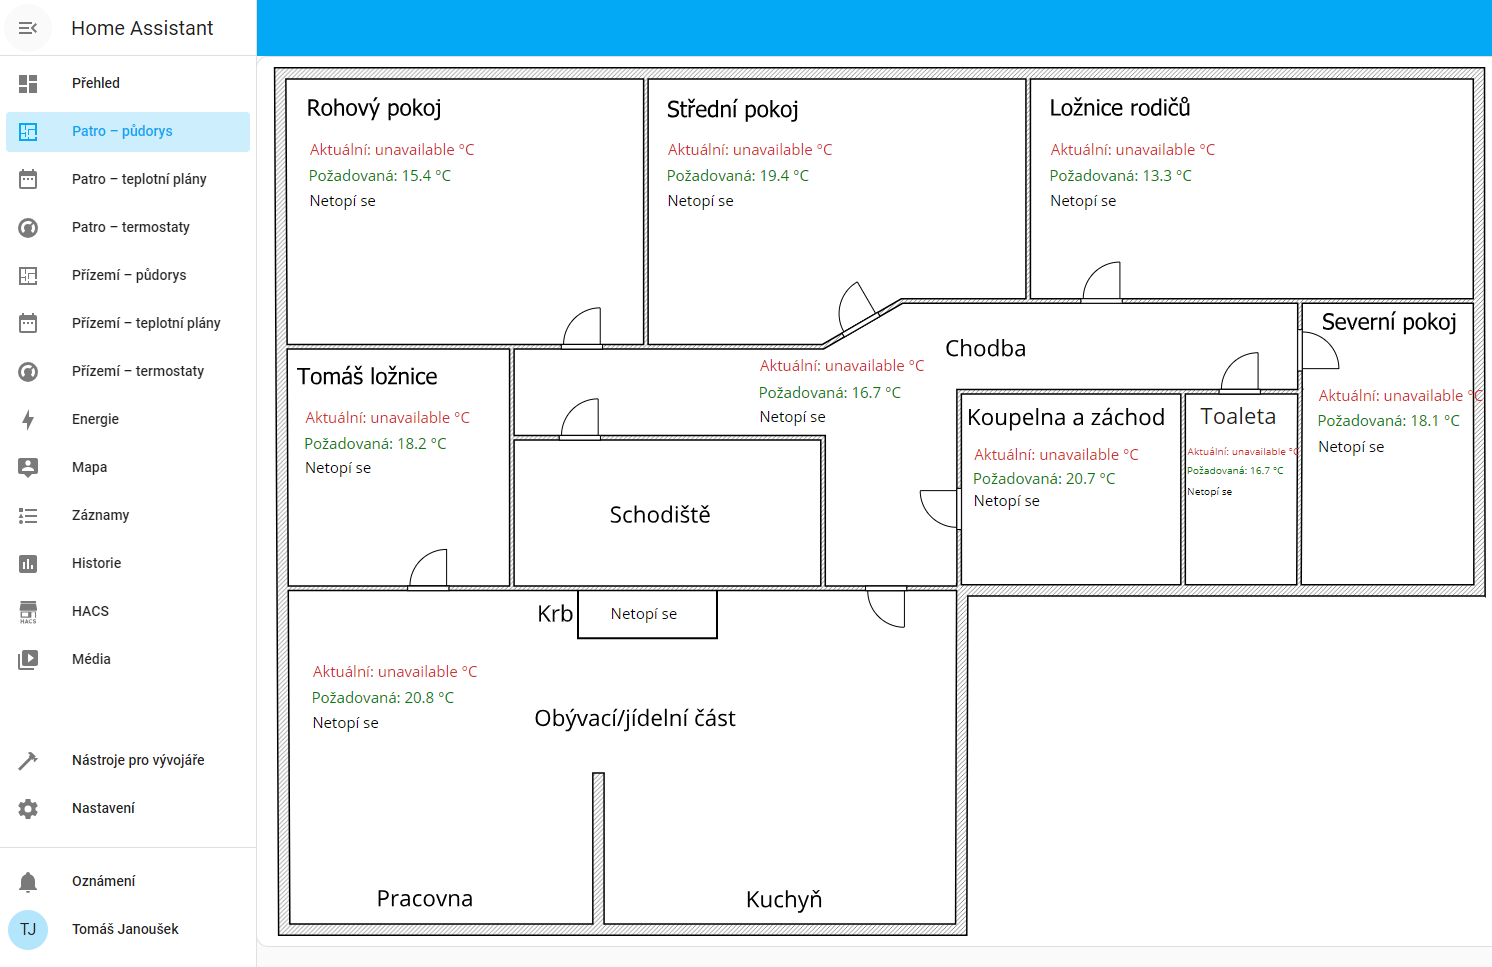
\includegraphics[width=1\textwidth]{pictures/czech/software/floor-plan-first-floor.png}
    \caption{Patro – půdorys.}
    \label{fig:floor-plan-first-floor}
\end{figure}
\end{Czech}
% ====================  STOP Devices Tab ====================